% Options for packages loaded elsewhere
\PassOptionsToPackage{unicode}{hyperref}
\PassOptionsToPackage{hyphens}{url}
%
\documentclass[
]{article}
\usepackage{lmodern}
\usepackage{amssymb,amsmath}
\usepackage{ifxetex,ifluatex}
\ifnum 0\ifxetex 1\fi\ifluatex 1\fi=0 % if pdftex
  \usepackage[T1]{fontenc}
  \usepackage[utf8]{inputenc}
  \usepackage{textcomp} % provide euro and other symbols
\else % if luatex or xetex
  \usepackage{unicode-math}
  \defaultfontfeatures{Scale=MatchLowercase}
  \defaultfontfeatures[\rmfamily]{Ligatures=TeX,Scale=1}
\fi
% Use upquote if available, for straight quotes in verbatim environments
\IfFileExists{upquote.sty}{\usepackage{upquote}}{}
\IfFileExists{microtype.sty}{% use microtype if available
  \usepackage[]{microtype}
  \UseMicrotypeSet[protrusion]{basicmath} % disable protrusion for tt fonts
}{}
\makeatletter
\@ifundefined{KOMAClassName}{% if non-KOMA class
  \IfFileExists{parskip.sty}{%
    \usepackage{parskip}
  }{% else
    \setlength{\parindent}{0pt}
    \setlength{\parskip}{6pt plus 2pt minus 1pt}}
}{% if KOMA class
  \KOMAoptions{parskip=half}}
\makeatother
\usepackage{xcolor}
\IfFileExists{xurl.sty}{\usepackage{xurl}}{} % add URL line breaks if available
\IfFileExists{bookmark.sty}{\usepackage{bookmark}}{\usepackage{hyperref}}
\hypersetup{
  pdftitle={STOR 455 Homework \#5},
  hidelinks,
  pdfcreator={LaTeX via pandoc}}
\urlstyle{same} % disable monospaced font for URLs
\usepackage[margin = 2.25cm]{geometry}
\usepackage{color}
\usepackage{fancyvrb}
\newcommand{\VerbBar}{|}
\newcommand{\VERB}{\Verb[commandchars=\\\{\}]}
\DefineVerbatimEnvironment{Highlighting}{Verbatim}{commandchars=\\\{\}}
% Add ',fontsize=\small' for more characters per line
\usepackage{framed}
\definecolor{shadecolor}{RGB}{248,248,248}
\newenvironment{Shaded}{\begin{snugshade}}{\end{snugshade}}
\newcommand{\AlertTok}[1]{\textcolor[rgb]{0.94,0.16,0.16}{#1}}
\newcommand{\AnnotationTok}[1]{\textcolor[rgb]{0.56,0.35,0.01}{\textbf{\textit{#1}}}}
\newcommand{\AttributeTok}[1]{\textcolor[rgb]{0.77,0.63,0.00}{#1}}
\newcommand{\BaseNTok}[1]{\textcolor[rgb]{0.00,0.00,0.81}{#1}}
\newcommand{\BuiltInTok}[1]{#1}
\newcommand{\CharTok}[1]{\textcolor[rgb]{0.31,0.60,0.02}{#1}}
\newcommand{\CommentTok}[1]{\textcolor[rgb]{0.56,0.35,0.01}{\textit{#1}}}
\newcommand{\CommentVarTok}[1]{\textcolor[rgb]{0.56,0.35,0.01}{\textbf{\textit{#1}}}}
\newcommand{\ConstantTok}[1]{\textcolor[rgb]{0.00,0.00,0.00}{#1}}
\newcommand{\ControlFlowTok}[1]{\textcolor[rgb]{0.13,0.29,0.53}{\textbf{#1}}}
\newcommand{\DataTypeTok}[1]{\textcolor[rgb]{0.13,0.29,0.53}{#1}}
\newcommand{\DecValTok}[1]{\textcolor[rgb]{0.00,0.00,0.81}{#1}}
\newcommand{\DocumentationTok}[1]{\textcolor[rgb]{0.56,0.35,0.01}{\textbf{\textit{#1}}}}
\newcommand{\ErrorTok}[1]{\textcolor[rgb]{0.64,0.00,0.00}{\textbf{#1}}}
\newcommand{\ExtensionTok}[1]{#1}
\newcommand{\FloatTok}[1]{\textcolor[rgb]{0.00,0.00,0.81}{#1}}
\newcommand{\FunctionTok}[1]{\textcolor[rgb]{0.00,0.00,0.00}{#1}}
\newcommand{\ImportTok}[1]{#1}
\newcommand{\InformationTok}[1]{\textcolor[rgb]{0.56,0.35,0.01}{\textbf{\textit{#1}}}}
\newcommand{\KeywordTok}[1]{\textcolor[rgb]{0.13,0.29,0.53}{\textbf{#1}}}
\newcommand{\NormalTok}[1]{#1}
\newcommand{\OperatorTok}[1]{\textcolor[rgb]{0.81,0.36,0.00}{\textbf{#1}}}
\newcommand{\OtherTok}[1]{\textcolor[rgb]{0.56,0.35,0.01}{#1}}
\newcommand{\PreprocessorTok}[1]{\textcolor[rgb]{0.56,0.35,0.01}{\textit{#1}}}
\newcommand{\RegionMarkerTok}[1]{#1}
\newcommand{\SpecialCharTok}[1]{\textcolor[rgb]{0.00,0.00,0.00}{#1}}
\newcommand{\SpecialStringTok}[1]{\textcolor[rgb]{0.31,0.60,0.02}{#1}}
\newcommand{\StringTok}[1]{\textcolor[rgb]{0.31,0.60,0.02}{#1}}
\newcommand{\VariableTok}[1]{\textcolor[rgb]{0.00,0.00,0.00}{#1}}
\newcommand{\VerbatimStringTok}[1]{\textcolor[rgb]{0.31,0.60,0.02}{#1}}
\newcommand{\WarningTok}[1]{\textcolor[rgb]{0.56,0.35,0.01}{\textbf{\textit{#1}}}}
\usepackage{graphicx,grffile}
\makeatletter
\def\maxwidth{\ifdim\Gin@nat@width>\linewidth\linewidth\else\Gin@nat@width\fi}
\def\maxheight{\ifdim\Gin@nat@height>\textheight\textheight\else\Gin@nat@height\fi}
\makeatother
% Scale images if necessary, so that they will not overflow the page
% margins by default, and it is still possible to overwrite the defaults
% using explicit options in \includegraphics[width, height, ...]{}
\setkeys{Gin}{width=\maxwidth,height=\maxheight,keepaspectratio}
% Set default figure placement to htbp
\makeatletter
\def\fps@figure{htbp}
\makeatother
\setlength{\emergencystretch}{3em} % prevent overfull lines
\providecommand{\tightlist}{%
  \setlength{\itemsep}{0pt}\setlength{\parskip}{0pt}}
\setcounter{secnumdepth}{-\maxdimen} % remove section numbering

\title{STOR 455 Homework \#5}
\usepackage{etoolbox}
\makeatletter
\providecommand{\subtitle}[1]{% add subtitle to \maketitle
  \apptocmd{\@title}{\par {\large #1 \par}}{}{}
}
\makeatother
\subtitle{40 points - Due 10/20 at 5:00pm}
\author{}
\date{\vspace{-2.5em}}

\begin{document}
\maketitle

\textbf{Directions:} For parts 6 and 9 you may work together, but they
should be \textbf{submitted individually} by each group member. For
parts 7 and 8, you should have only \textbf{one submission per group}.
There will be separate places on Gradescope to submit the individual vs
group work.

\textbf{Situation:} Can we predict the selling price of a house in Ames,
Iowa based on recorded features of the house? That is your task for this
assignment. Each team will get a dataset with information on forty
potential predictors and the selling price (in \$1,000's) for a sample
of homes. The data sets for your group are AmesTrain??.csv and
AmesTest??.csv (where ?? corresponds to your group number) A separate
file identifies the variables in the Ames Housing data and explains some
of the coding.

\begin{Shaded}
\begin{Highlighting}[]
\KeywordTok{library}\NormalTok{(readr)}
\KeywordTok{library}\NormalTok{(corrplot)}
\end{Highlighting}
\end{Shaded}

\begin{verbatim}
## corrplot 0.90 loaded
\end{verbatim}

\begin{Shaded}
\begin{Highlighting}[]
\KeywordTok{library}\NormalTok{(leaps)}
\KeywordTok{library}\NormalTok{(car)}
\end{Highlighting}
\end{Shaded}

\begin{verbatim}
## Loading required package: carData
\end{verbatim}

\hypertarget{part-6.-cross-validation}{%
\paragraph{Part 6. Cross-validation:}\label{part-6.-cross-validation}}

In some situations, a model might fit the peculiarities of a specific
sample of data well, but not reflect structure that is really present in
the population. A good test for how your model might work on ``real''
house prices can be simulated by seeing how well your fitted model does
at predicting prices that were NOT in your original sample. This is why
we reserved an additional 200 cases as a holdout sample in
AmesTest??.csv. Import your holdout test data and

\begin{Shaded}
\begin{Highlighting}[]
\KeywordTok{setwd}\NormalTok{(}\StringTok{"C:/Users/adeve/Desktop"}\NormalTok{)}
\NormalTok{amestrain24 <-}\StringTok{ }\KeywordTok{read.csv}\NormalTok{(}\StringTok{"AmesTrain24.csv"}\NormalTok{)}
\NormalTok{amestest24 <-}\StringTok{ }\KeywordTok{read.csv}\NormalTok{(}\StringTok{"AmesTest24.csv"}\NormalTok{)}
\end{Highlighting}
\end{Shaded}

\begin{itemize}
\tightlist
\item
  Compute the predicted Price for each of the cases in the holdout test
  sample, using your model resulting from the initial fit and residual
  analysis in parts 1 and 2 of Homework \#3. This should be done with
  the same AmesTrain??.csv dataset that you used for homework \#3, with
  your assignment \#3 group numbe, and AmesTrain?? also using your
  assignment \#3 group number.
\end{itemize}

\begin{Shaded}
\begin{Highlighting}[]
\NormalTok{allsubmod =}\StringTok{ }\KeywordTok{lm}\NormalTok{(Price}\OperatorTok{~}\NormalTok{Fireplaces}\OperatorTok{+}\NormalTok{GarageSF}\OperatorTok{+}\NormalTok{GroundSF, amestrain24)}

\NormalTok{ames.test.predict <-}\StringTok{ }\KeywordTok{predict}\NormalTok{(allsubmod, }\DataTypeTok{newdata=}\NormalTok{amestest24)}
\end{Highlighting}
\end{Shaded}

\begin{itemize}
\tightlist
\item
  Compute the residuals for the 200 holdout cases.
\end{itemize}

\begin{Shaded}
\begin{Highlighting}[]
\NormalTok{ames.test.residual =}\StringTok{ }\NormalTok{amestest24}\OperatorTok{$}\NormalTok{Price }\OperatorTok{-}\StringTok{ }\NormalTok{ames.test.predict}
\end{Highlighting}
\end{Shaded}

\begin{itemize}
\tightlist
\item
  Compute the mean and standard deviation of these residuals. Are they
  close to what you expect from the training model?
\end{itemize}

\emph{From the summary of the allsubmod, we would expect a residual
standard error of 46.14. Since the ames.test.residual is 37.61 and we
are talking about thousands of dollars when referring to houses, the
residual is roughly close enough to what we would expect from the
training model.}

\begin{Shaded}
\begin{Highlighting}[]
\KeywordTok{mean}\NormalTok{(ames.test.residual)}
\end{Highlighting}
\end{Shaded}

\begin{verbatim}
## [1] 4.265713
\end{verbatim}

\begin{Shaded}
\begin{Highlighting}[]
\KeywordTok{sd}\NormalTok{(ames.test.residual)}
\end{Highlighting}
\end{Shaded}

\begin{verbatim}
## [1] 37.61052
\end{verbatim}

\begin{Shaded}
\begin{Highlighting}[]
\KeywordTok{summary}\NormalTok{(allsubmod)}
\end{Highlighting}
\end{Shaded}

\begin{verbatim}
## 
## Call:
## lm(formula = Price ~ Fireplaces + GarageSF + GroundSF, data = amestrain24)
## 
## Residuals:
##      Min       1Q   Median       3Q      Max 
## -189.853  -26.864   -1.401   21.907  233.684 
## 
## Coefficients:
##              Estimate Std. Error t value Pr(>|t|)    
## (Intercept)  6.891286   6.291353   1.095    0.274    
## Fireplaces  19.901124   3.513306   5.665  2.3e-08 ***
## GarageSF     0.142456   0.009959  14.305  < 2e-16 ***
## GroundSF     0.062734   0.004650  13.490  < 2e-16 ***
## ---
## Signif. codes:  0 '***' 0.001 '**' 0.01 '*' 0.05 '.' 0.1 ' ' 1
## 
## Residual standard error: 46.14 on 596 degrees of freedom
## Multiple R-squared:  0.6301, Adjusted R-squared:  0.6283 
## F-statistic: 338.5 on 3 and 596 DF,  p-value: < 2.2e-16
\end{verbatim}

\begin{itemize}
\tightlist
\item
  Construct a plot of the residuals to determine if they are normally
  distributed. Is this plot what you expect to see considering the
  training model? \emph{The residuals in the testing data are more
  spread out than in the training data. Furthermore, the right tail of
  the QQNorm plot on the testing data is much more prominent than the
  training data. This suggests that there may be a skew that a model
  that is fitted to the testing data that may not be accounted for in
  the other data.}
\end{itemize}

\begin{Shaded}
\begin{Highlighting}[]
\KeywordTok{plot}\NormalTok{(allsubmod)}
\end{Highlighting}
\end{Shaded}

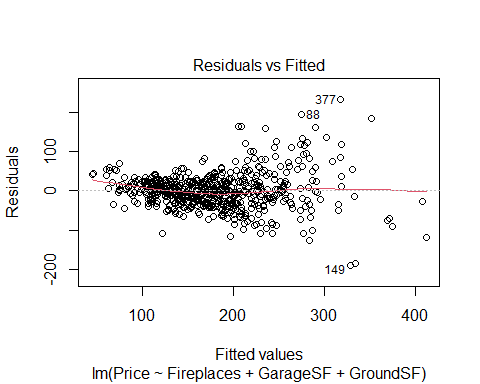
\includegraphics{Homework-5.3_files/figure-latex/unnamed-chunk-6-1.pdf}
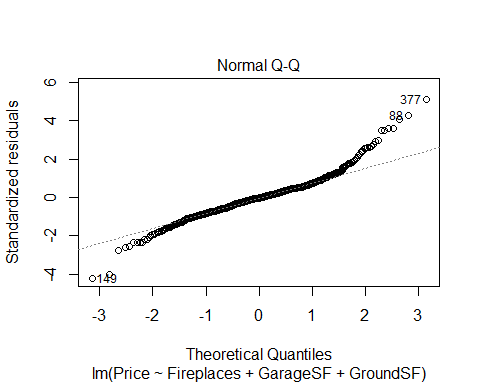
\includegraphics{Homework-5.3_files/figure-latex/unnamed-chunk-6-2.pdf}
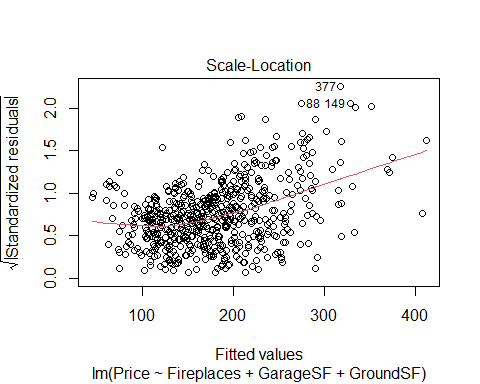
\includegraphics{Homework-5.3_files/figure-latex/unnamed-chunk-6-3.pdf}
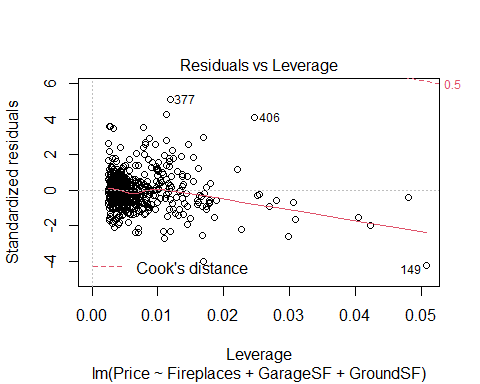
\includegraphics{Homework-5.3_files/figure-latex/unnamed-chunk-6-4.pdf}

\begin{Shaded}
\begin{Highlighting}[]
\KeywordTok{hist}\NormalTok{(allsubmod}\OperatorTok{$}\NormalTok{residuals)}
\end{Highlighting}
\end{Shaded}

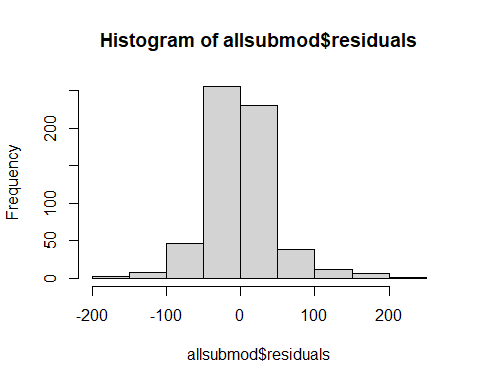
\includegraphics{Homework-5.3_files/figure-latex/unnamed-chunk-6-5.pdf}

\begin{Shaded}
\begin{Highlighting}[]
\KeywordTok{plot}\NormalTok{(ames.test.residual)}
\end{Highlighting}
\end{Shaded}

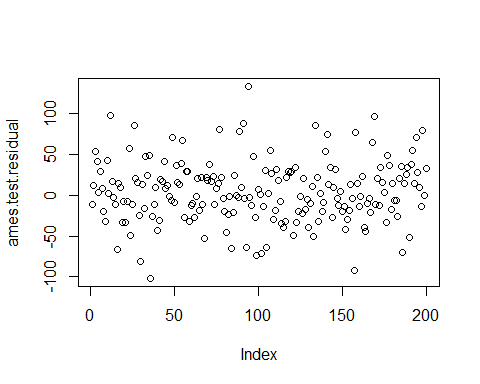
\includegraphics{Homework-5.3_files/figure-latex/unnamed-chunk-6-6.pdf}

\begin{Shaded}
\begin{Highlighting}[]
\KeywordTok{qqnorm}\NormalTok{(ames.test.residual)}
\KeywordTok{qqline}\NormalTok{(ames.test.residual)}
\end{Highlighting}
\end{Shaded}

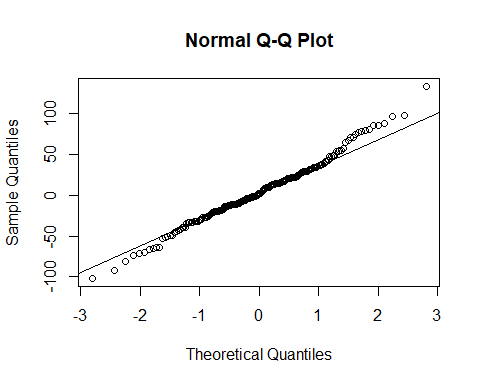
\includegraphics{Homework-5.3_files/figure-latex/unnamed-chunk-6-7.pdf}

\begin{Shaded}
\begin{Highlighting}[]
\KeywordTok{hist}\NormalTok{(ames.test.residual)}
\end{Highlighting}
\end{Shaded}

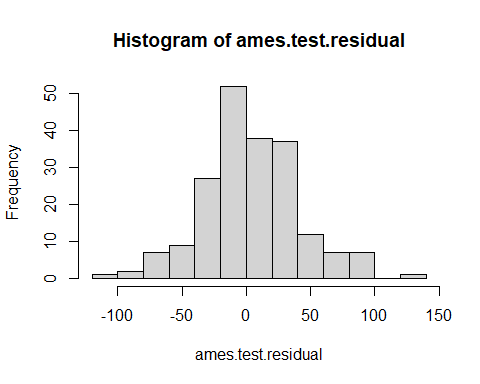
\includegraphics{Homework-5.3_files/figure-latex/unnamed-chunk-6-8.pdf}

\begin{itemize}
\tightlist
\item
  Are any holdout cases especially poorly predicted by the training
  model? If so, identify by the row number(s) in the holdout data.
  \emph{The biggest holdout case is 94 with a residual value of positive
  133.758. Based on the cook's distance plot in the previous question,
  there does not appear to be any points outside of 0.5 of cook's
  distance, so that is good.}
\end{itemize}

\begin{Shaded}
\begin{Highlighting}[]
\KeywordTok{head}\NormalTok{(}\KeywordTok{sort}\NormalTok{(ames.test.residual), }\DataTypeTok{decreasing=}\OtherTok{FALSE}\NormalTok{, }\DecValTok{10}\NormalTok{)}
\end{Highlighting}
\end{Shaded}

\begin{verbatim}
##         36        157         30         99        102        186         16 
## -101.95333  -91.94209  -81.53233  -73.62176  -71.50196  -69.83581  -66.29810 
##         84         93        105 
##  -65.74621  -64.22883  -63.97843
\end{verbatim}

\begin{Shaded}
\begin{Highlighting}[]
\KeywordTok{tail}\NormalTok{(}\KeywordTok{sort}\NormalTok{(ames.test.residual), }\DataTypeTok{decreasing=}\OtherTok{TRUE}\NormalTok{, }\DecValTok{10}\NormalTok{)}
\end{Highlighting}
\end{Shaded}

\begin{verbatim}
##       158        89       198        77       134        26        91       169 
##  76.78719  78.43109  80.17102  80.82564  85.24867  86.12330  88.21376  96.82794 
##        12        94 
##  98.54538 133.75848
\end{verbatim}

\begin{itemize}
\tightlist
\item
  Compute the correlation between the predicted values and actual prices
  for the holdout sample. This is known as the cross-validation
  correlation. We don't expect the training model to do better at
  predicting values different from those that were used to build it (as
  reflected in the original \(R^{2}\)), but an effective model shouldn't
  do a lot worse at predicting the holdout values. Square the
  cross-validation correlation to get an \(R^{2}\) value and subtract it
  from the original \(R^{2}\) of the training sample. This is known as
  the shrinkage. We won't have specific rules about how little the
  shrinkage should be, but give an opinion on whether the shrinkage
  looks OK to you or too large in your situation.
\end{itemize}

\emph{The shrinkage is 0.3279954, which is pretty bad It could
definitely be better. If it was closer to 0, it would mean that the
model is going a better job at predicting the new data compared to the
original data. We should aim for a shrinkage under 1\%, and this is at
least 32\%, which is pretty bad.}

\begin{Shaded}
\begin{Highlighting}[]
\NormalTok{crosscor =}\StringTok{ }\KeywordTok{cor}\NormalTok{(amestest24}\OperatorTok{$}\NormalTok{Price, ames.test.residual)}

\KeywordTok{summary}\NormalTok{(allsubmod)}\OperatorTok{$}\NormalTok{r.squared}
\end{Highlighting}
\end{Shaded}

\begin{verbatim}
## [1] 0.6301369
\end{verbatim}

\begin{Shaded}
\begin{Highlighting}[]
\NormalTok{crosscor}\OperatorTok{^}\DecValTok{2}
\end{Highlighting}
\end{Shaded}

\begin{verbatim}
## [1] 0.3021415
\end{verbatim}

\begin{Shaded}
\begin{Highlighting}[]
\NormalTok{Shrinkage =}\StringTok{ }\KeywordTok{summary}\NormalTok{(allsubmod)}\OperatorTok{$}\NormalTok{r.squared }\OperatorTok{-}\StringTok{ }\NormalTok{crosscor}\OperatorTok{^}\DecValTok{2}
\NormalTok{Shrinkage}
\end{Highlighting}
\end{Shaded}

\begin{verbatim}
## [1] 0.3279954
\end{verbatim}

\hypertarget{part-7.-find-a-fancy-model}{%
\paragraph{Part 7. Find a ``fancy
model'':}\label{part-7.-find-a-fancy-model}}

Use AmesTrain??.csv, where ?? corresponds to your new group number. In
addition to the quantitative predictors from homework \#3, you may now
consider models with

\begin{itemize}
\item
  Categorical variables from the original dataset. Just put these in the
  model and let R take care of making the indicator predictors (and
  picking one category to leave out). Use factor( ) to treat a numeric
  variable as categorical. You'll see the coefficients for each
  indicator when you look at the summary( ) and they will be grouped
  together in the ANOVA. Be careful, since adding a single categorical
  variable with a lot of categories might actually be adding a lot of
  new indicator terms.
\item
  Transformations of predictors. You can include functions of
  quantitative predictors. Probably best to use the I( ) notation so you
  don't need to create new columns when you run the predictions for the
  test data.
\item
  Transformations of the response. You might address curvature or
  skewness in residual plots by transforming the response prices with a
  function like log(Price), sqrt(Price), Price\^{}2, etc.. These should
  generally not need the I( ) notation to make these adjustments.
  IMPORTANT: If you transform Price, be sure to reverse the
  transformation when making final predictions!
\item
  Combinations of variables. This might include interactions or other
  combinations. You do not need the I( ) notation when making an
  interaction using a categorical predictor (e.g.~GroundSF*CentralAir).
\end{itemize}

Keep general track of the approaches you try and explain what guides
your decisions as you select a new set of predictors (but again you
don't need to give full details of every model you consider). Along the
way you should consider some residual analysis.

\begin{Shaded}
\begin{Highlighting}[]
\NormalTok{AmesTest5 <-}\StringTok{ }\KeywordTok{read.csv}\NormalTok{(}\StringTok{"AmesTest5.csv"}\NormalTok{)}
\NormalTok{AmesTrain5 <-}\StringTok{ }\KeywordTok{read.csv}\NormalTok{(}\StringTok{"AmesTrain5.csv"}\NormalTok{)}
\end{Highlighting}
\end{Shaded}

Our full model from Homework 3 was:

\begin{Shaded}
\begin{Highlighting}[]
\NormalTok{AmesTrain5}\OperatorTok{$}\NormalTok{HBath =}\StringTok{ }\NormalTok{AmesTrain5}\OperatorTok{$}\NormalTok{BasementHBath }\OperatorTok{+}\StringTok{ }\NormalTok{AmesTrain5}\OperatorTok{$}\NormalTok{HalfBath}
\NormalTok{AmesTrain5}\OperatorTok{$}\NormalTok{FBath =}\StringTok{ }\NormalTok{AmesTrain5}\OperatorTok{$}\NormalTok{BasementFBath }\OperatorTok{+}\StringTok{ }\NormalTok{AmesTrain5}\OperatorTok{$}\NormalTok{FullBath}
\NormalTok{AmesTrain5}\OperatorTok{$}\NormalTok{Porch =}\StringTok{ }\NormalTok{AmesTrain5}\OperatorTok{$}\NormalTok{OpenPorchSF }\OperatorTok{+}\StringTok{ }\NormalTok{AmesTrain5}\OperatorTok{$}\NormalTok{EnclosedPorchSF }\OperatorTok{+}\StringTok{ }\NormalTok{AmesTrain5}\OperatorTok{$}\NormalTok{ScreenPorchSF}

\NormalTok{HW3Full =}\StringTok{ }\KeywordTok{lm}\NormalTok{(}\DataTypeTok{formula =} \KeywordTok{log}\NormalTok{(Price) }\OperatorTok{~}\StringTok{ }\NormalTok{YearBuilt }\OperatorTok{+}\StringTok{ }\NormalTok{YearRemodel }\OperatorTok{+}\StringTok{ }\NormalTok{LotFrontage }\OperatorTok{+}\StringTok{ }\KeywordTok{I}\NormalTok{(}\KeywordTok{log}\NormalTok{(LotArea)) }\OperatorTok{+}\StringTok{ }\NormalTok{Quality }\OperatorTok{+}\StringTok{ }\NormalTok{Condition }\OperatorTok{+}\StringTok{ }\NormalTok{BasementFinSF }\OperatorTok{+}\StringTok{ }\NormalTok{BasementUnFinSF }\OperatorTok{+}\StringTok{ }\NormalTok{BasementSF }\OperatorTok{+}\StringTok{ }\NormalTok{FirstSF }\OperatorTok{+}\StringTok{ }\NormalTok{SecondSF }\OperatorTok{+}\StringTok{ }\KeywordTok{I}\NormalTok{(}\KeywordTok{log}\NormalTok{(GroundSF)) }\OperatorTok{+}\StringTok{ }\NormalTok{Bedroom }\OperatorTok{+}\StringTok{ }\NormalTok{TotalRooms }\OperatorTok{+}\StringTok{ }\NormalTok{Fireplaces }\OperatorTok{+}\StringTok{ }\NormalTok{GarageCars }\OperatorTok{+}\StringTok{ }\KeywordTok{I}\NormalTok{(GarageSF}\OperatorTok{^}\FloatTok{1.5}\NormalTok{) }\OperatorTok{+}\StringTok{ }\NormalTok{WoodDeckSF }\OperatorTok{+}\StringTok{ }\NormalTok{HBath }\OperatorTok{+}\StringTok{ }\NormalTok{FBath }\OperatorTok{+}\StringTok{ }\NormalTok{Porch,}
                 \DataTypeTok{data =}\NormalTok{ AmesTrain5)}
\end{Highlighting}
\end{Shaded}

So to begin, we transformed the same predictors and our response
variable for our initial full model here. Additionally, we used the same
combinations of variables: HBath, FBath, and Porch. We then added into
our full model all of the categorical predictors.

\begin{Shaded}
\begin{Highlighting}[]
\NormalTok{FullTest =}\StringTok{ }\KeywordTok{lm}\NormalTok{(}\KeywordTok{log}\NormalTok{(Price)}\OperatorTok{~}
\StringTok{            }\NormalTok{LotConfig }\OperatorTok{+}\StringTok{ }\NormalTok{HouseStyle }\OperatorTok{+}\StringTok{ }\NormalTok{ExteriorQ }\OperatorTok{+}\StringTok{ }\NormalTok{ExteriorC }\OperatorTok{+}\StringTok{ }\NormalTok{Foundation }\OperatorTok{+}\StringTok{ }\NormalTok{BasementHt }\OperatorTok{+}\StringTok{ }\NormalTok{BasementC }\OperatorTok{+}\StringTok{ }\NormalTok{BasementFin }\OperatorTok{+}\StringTok{ }\NormalTok{Heating }\OperatorTok{+}\StringTok{ }\NormalTok{HeatingQC }\OperatorTok{+}\StringTok{ }\NormalTok{CentralAir }\OperatorTok{+}\StringTok{ }\NormalTok{KitchenQ }\OperatorTok{+}\StringTok{ }\NormalTok{GarageType }\OperatorTok{+}\StringTok{ }\NormalTok{GarageQ }\OperatorTok{+}\StringTok{ }\NormalTok{GarageC }\OperatorTok{+}\StringTok{ }\NormalTok{YearBuilt }\OperatorTok{+}\StringTok{ }\NormalTok{YearRemodel }\OperatorTok{+}\StringTok{ }\NormalTok{LotFrontage }\OperatorTok{+}\StringTok{ }\KeywordTok{I}\NormalTok{(}\KeywordTok{log}\NormalTok{(LotArea)) }\OperatorTok{+}\StringTok{ }\KeywordTok{factor}\NormalTok{(Quality) }\OperatorTok{+}\StringTok{ }\KeywordTok{factor}\NormalTok{(Condition) }\OperatorTok{+}\StringTok{ }\NormalTok{BasementFinSF }\OperatorTok{+}\StringTok{ }\NormalTok{BasementUnFinSF }\OperatorTok{+}\StringTok{ }\NormalTok{BasementSF }\OperatorTok{+}\StringTok{ }\NormalTok{FirstSF }\OperatorTok{+}\StringTok{ }\NormalTok{SecondSF }\OperatorTok{+}\StringTok{ }\KeywordTok{I}\NormalTok{(}\KeywordTok{log}\NormalTok{(GroundSF)) }\OperatorTok{+}\StringTok{ }\NormalTok{Bedroom }\OperatorTok{+}\StringTok{ }\NormalTok{TotalRooms }\OperatorTok{+}\StringTok{ }\NormalTok{Fireplaces }\OperatorTok{+}\StringTok{ }\NormalTok{GarageCars }\OperatorTok{+}\StringTok{ }\KeywordTok{I}\NormalTok{(GarageSF}\OperatorTok{^}\FloatTok{1.5}\NormalTok{) }\OperatorTok{+}\StringTok{ }\NormalTok{WoodDeckSF }\OperatorTok{+}\StringTok{ }\NormalTok{HBath }\OperatorTok{+}\StringTok{ }\NormalTok{FBath }\OperatorTok{+}\StringTok{ }\NormalTok{Porch, }\DataTypeTok{data=}\NormalTok{AmesTrain5)}

\KeywordTok{plot}\NormalTok{(FullTest)[}\DecValTok{1}\OperatorTok{:}\DecValTok{2}\NormalTok{]}
\end{Highlighting}
\end{Shaded}

\begin{verbatim}
## Warning: not plotting observations with leverage one:
##   30, 50, 176, 187, 233, 398, 425, 482, 581, 585
\end{verbatim}

\includegraphics{Homework-5.3_files/figure-latex/unnamed-chunk-11-1.pdf}
\includegraphics{Homework-5.3_files/figure-latex/unnamed-chunk-11-2.pdf}
\includegraphics{Homework-5.3_files/figure-latex/unnamed-chunk-11-3.pdf}
\includegraphics{Homework-5.3_files/figure-latex/unnamed-chunk-11-4.pdf}

\begin{verbatim}
## NULL
\end{verbatim}

\begin{Shaded}
\begin{Highlighting}[]
\CommentTok{#what does error message mean}
\end{Highlighting}
\end{Shaded}

1st Full model with initial predictor pool:

\begin{Shaded}
\begin{Highlighting}[]
\NormalTok{Full =}\StringTok{ }\KeywordTok{lm}\NormalTok{(}\KeywordTok{log}\NormalTok{(Price)}\OperatorTok{~}
\StringTok{            }\NormalTok{LotConfig }\OperatorTok{+}\StringTok{ }\NormalTok{HouseStyle }\OperatorTok{+}\StringTok{ }\NormalTok{ExteriorQ }\OperatorTok{+}\StringTok{ }\NormalTok{ExteriorC }\OperatorTok{+}\StringTok{ }\NormalTok{Foundation }\OperatorTok{+}\StringTok{ }\NormalTok{BasementHt }\OperatorTok{+}\StringTok{ }\NormalTok{BasementC }\OperatorTok{+}\StringTok{ }\NormalTok{BasementFin }\OperatorTok{+}\StringTok{ }\NormalTok{Heating }\OperatorTok{+}\StringTok{ }\NormalTok{HeatingQC }\OperatorTok{+}\StringTok{ }\NormalTok{CentralAir }\OperatorTok{+}\StringTok{ }\NormalTok{KitchenQ }\OperatorTok{+}\StringTok{ }\NormalTok{GarageType }\OperatorTok{+}\StringTok{ }\NormalTok{GarageQ }\OperatorTok{+}\StringTok{ }\NormalTok{GarageC }\OperatorTok{+}\StringTok{ }\NormalTok{YearBuilt }\OperatorTok{+}\StringTok{ }\NormalTok{YearRemodel }\OperatorTok{+}\StringTok{ }\NormalTok{LotFrontage }\OperatorTok{+}\StringTok{ }\KeywordTok{I}\NormalTok{(}\KeywordTok{log}\NormalTok{(LotArea)) }\OperatorTok{+}\StringTok{ }\KeywordTok{factor}\NormalTok{(Quality) }\OperatorTok{+}\StringTok{ }\KeywordTok{factor}\NormalTok{(Condition) }\OperatorTok{+}\StringTok{ }\NormalTok{BasementFinSF }\OperatorTok{+}\StringTok{ }\NormalTok{BasementUnFinSF }\OperatorTok{+}\StringTok{ }\NormalTok{BasementSF }\OperatorTok{+}\StringTok{ }\NormalTok{FirstSF }\OperatorTok{+}\StringTok{ }\NormalTok{SecondSF }\OperatorTok{+}\StringTok{ }\KeywordTok{I}\NormalTok{(}\KeywordTok{log}\NormalTok{(GroundSF)) }\OperatorTok{+}\StringTok{ }\NormalTok{Bedroom }\OperatorTok{+}\StringTok{ }\NormalTok{TotalRooms }\OperatorTok{+}\StringTok{ }\NormalTok{Fireplaces }\OperatorTok{+}\StringTok{ }\NormalTok{GarageCars }\OperatorTok{+}\StringTok{ }\KeywordTok{I}\NormalTok{(GarageSF}\OperatorTok{^}\FloatTok{1.5}\NormalTok{) }\OperatorTok{+}\StringTok{ }\NormalTok{WoodDeckSF }\OperatorTok{+}\StringTok{ }\NormalTok{HBath }\OperatorTok{+}\StringTok{ }\NormalTok{FBath }\OperatorTok{+}\StringTok{ }\NormalTok{Porch }\OperatorTok{+}\StringTok{ }\NormalTok{WoodDeckSF}\OperatorTok{*}\NormalTok{Porch }\OperatorTok{+}\StringTok{ }\KeywordTok{factor}\NormalTok{(Quality)}\OperatorTok{*}\NormalTok{YearBuilt }\OperatorTok{+}\StringTok{ }\KeywordTok{factor}\NormalTok{(Quality)}\OperatorTok{*}\NormalTok{YearRemodel }\OperatorTok{+}\StringTok{ }\KeywordTok{factor}\NormalTok{(Condition)}\OperatorTok{*}\NormalTok{YearBuilt }\OperatorTok{+}\StringTok{ }\KeywordTok{factor}\NormalTok{(Condition)}\OperatorTok{*}\NormalTok{YearRemodel, }\DataTypeTok{data=}\NormalTok{AmesTrain5)}
\end{Highlighting}
\end{Shaded}

Fist, we applied factor() to the Quality and Condition predictors, as
while they are numeric, they are more accurately described as
categorical variables since they group homes into one of 10 categories.

We added an interaction term between: -WoodDeckSF and Porch predictors
because they are both related to outdoor space -factor(Quality) and
YearBuilt and YearRemodel because how old a house is/when a house was
updated often means it is of a better quality -factor(Condition) and
YearBuilt and YearRemodel because how old a house is/when a house was
updated often means it is in better condition

Next, we used Forward Selection, Stepwise Regression, and Backwards
Elimination and compared each output's AIC to determine which was the
best model from this predictor pool.

Forward Selection:

\begin{Shaded}
\begin{Highlighting}[]
\NormalTok{none =}\StringTok{ }\KeywordTok{lm}\NormalTok{(}\KeywordTok{log}\NormalTok{(Price)}\OperatorTok{~}\DecValTok{1}\NormalTok{, }\DataTypeTok{data=}\NormalTok{AmesTrain5)}

\NormalTok{MSE =}\StringTok{ }\NormalTok{(}\KeywordTok{summary}\NormalTok{(Full)}\OperatorTok{$}\NormalTok{sigma)}\OperatorTok{^}\DecValTok{2}

\KeywordTok{step}\NormalTok{(none, }\DataTypeTok{scope =} \KeywordTok{list}\NormalTok{(}\DataTypeTok{upper=}\NormalTok{Full), }\DataTypeTok{scale=}\NormalTok{MSE, }\DataTypeTok{direction =} \StringTok{'forward'}\NormalTok{, }\DataTypeTok{trace=}\OtherTok{FALSE}\NormalTok{)}
\end{Highlighting}
\end{Shaded}

\begin{verbatim}
## 
## Call:
## lm(formula = log(Price) ~ factor(Quality) + I(log(GroundSF)) + 
##     YearBuilt + I(log(LotArea)) + factor(Condition) + BasementFinSF + 
##     GarageCars + Porch + BasementSF + Fireplaces + KitchenQ + 
##     CentralAir + GarageC + HeatingQC + LotFrontage + SecondSF + 
##     HouseStyle + Bedroom + FirstSF + factor(Quality):YearBuilt + 
##     YearBuilt:factor(Condition), data = AmesTrain5)
## 
## Coefficients:
##                  (Intercept)              factor(Quality)2  
##                    3.249e+03                    -3.258e+03  
##             factor(Quality)3              factor(Quality)4  
##                   -3.258e+03                    -3.253e+03  
##             factor(Quality)5              factor(Quality)6  
##                   -3.254e+03                    -3.252e+03  
##             factor(Quality)7              factor(Quality)8  
##                   -3.251e+03                    -3.249e+03  
##             factor(Quality)9             factor(Quality)10  
##                   -3.282e+03                    -3.217e+03  
##             I(log(GroundSF))                     YearBuilt  
##                    2.243e-01                    -1.664e+00  
##              I(log(LotArea))            factor(Condition)2  
##                    9.068e-02                    -2.548e+00  
##           factor(Condition)3            factor(Condition)4  
##                    1.089e+01                     1.962e+00  
##           factor(Condition)5            factor(Condition)6  
##                   -3.774e+00                    -2.191e+00  
##           factor(Condition)7            factor(Condition)8  
##                    1.835e+00                    -1.436e-01  
##           factor(Condition)9                 BasementFinSF  
##                    2.981e-01                     7.596e-05  
##                   GarageCars                         Porch  
##                    4.094e-02                     1.642e-04  
##                   BasementSF                    Fireplaces  
##                    1.041e-04                     4.774e-02  
##                   KitchenQFa                    KitchenQGd  
##                   -1.338e-01                    -9.228e-02  
##                   KitchenQPo                    KitchenQTA  
##                   -1.239e-01                    -9.294e-02  
##                  CentralAirY                     GarageCFa  
##                    5.492e-02                     4.104e-03  
##                    GarageCGd                   GarageCNone  
##                    6.902e-02                    -1.426e-02  
##                    GarageCPo                     GarageCTA  
##                    2.533e-01                     4.340e-02  
##                  HeatingQCFa                   HeatingQCGd  
##                   -6.099e-02                    -1.511e-02  
##                  HeatingQCPo                   HeatingQCTA  
##                   -8.692e-02                    -4.100e-02  
##                  LotFrontage                      SecondSF  
##                    2.911e-04                     2.002e-04  
##             HouseStyle1.5Unf              HouseStyle1Story  
##                   -2.485e-02                     4.743e-02  
##             HouseStyle2.5Fin              HouseStyle2.5Unf  
##                   -1.455e-01                    -8.683e-02  
##             HouseStyle2Story              HouseStyleSFoyer  
##                   -6.371e-02                     1.473e-02  
##               HouseStyleSLvl                       Bedroom  
##                    1.218e-02                    -1.299e-02  
##                      FirstSF    factor(Quality)2:YearBuilt  
##                    7.567e-05                     1.669e+00  
##   factor(Quality)3:YearBuilt    factor(Quality)4:YearBuilt  
##                    1.670e+00                     1.667e+00  
##   factor(Quality)5:YearBuilt    factor(Quality)6:YearBuilt  
##                    1.668e+00                     1.667e+00  
##   factor(Quality)7:YearBuilt    factor(Quality)8:YearBuilt  
##                    1.667e+00                     1.666e+00  
##   factor(Quality)9:YearBuilt   factor(Quality)10:YearBuilt  
##                    1.682e+00                     1.650e+00  
## YearBuilt:factor(Condition)2  YearBuilt:factor(Condition)3  
##                    1.286e-03                    -5.560e-03  
## YearBuilt:factor(Condition)4  YearBuilt:factor(Condition)5  
##                   -9.819e-04                     1.985e-03  
## YearBuilt:factor(Condition)6  YearBuilt:factor(Condition)7  
##                    1.209e-03                    -8.269e-04  
## YearBuilt:factor(Condition)8  YearBuilt:factor(Condition)9  
##                    2.046e-04                            NA
\end{verbatim}

AIC=-62.6

Stepwise Regression:

\begin{Shaded}
\begin{Highlighting}[]
\KeywordTok{step}\NormalTok{(none, }\DataTypeTok{scope =} \KeywordTok{list}\NormalTok{(}\DataTypeTok{upper=}\NormalTok{Full), }\DataTypeTok{scale=}\NormalTok{MSE, }\DataTypeTok{trace=}\OtherTok{FALSE}\NormalTok{)}
\end{Highlighting}
\end{Shaded}

\begin{verbatim}
## 
## Call:
## lm(formula = log(Price) ~ factor(Quality) + I(log(GroundSF)) + 
##     YearBuilt + I(log(LotArea)) + factor(Condition) + BasementFinSF + 
##     GarageCars + Porch + BasementSF + Fireplaces + KitchenQ + 
##     CentralAir + GarageC + HeatingQC + LotFrontage + SecondSF + 
##     HouseStyle + Bedroom + FirstSF + factor(Quality):YearBuilt + 
##     YearBuilt:factor(Condition), data = AmesTrain5)
## 
## Coefficients:
##                  (Intercept)              factor(Quality)2  
##                    3.249e+03                    -3.258e+03  
##             factor(Quality)3              factor(Quality)4  
##                   -3.258e+03                    -3.253e+03  
##             factor(Quality)5              factor(Quality)6  
##                   -3.254e+03                    -3.252e+03  
##             factor(Quality)7              factor(Quality)8  
##                   -3.251e+03                    -3.249e+03  
##             factor(Quality)9             factor(Quality)10  
##                   -3.282e+03                    -3.217e+03  
##             I(log(GroundSF))                     YearBuilt  
##                    2.243e-01                    -1.664e+00  
##              I(log(LotArea))            factor(Condition)2  
##                    9.068e-02                    -2.548e+00  
##           factor(Condition)3            factor(Condition)4  
##                    1.089e+01                     1.962e+00  
##           factor(Condition)5            factor(Condition)6  
##                   -3.774e+00                    -2.191e+00  
##           factor(Condition)7            factor(Condition)8  
##                    1.835e+00                    -1.436e-01  
##           factor(Condition)9                 BasementFinSF  
##                    2.981e-01                     7.596e-05  
##                   GarageCars                         Porch  
##                    4.094e-02                     1.642e-04  
##                   BasementSF                    Fireplaces  
##                    1.041e-04                     4.774e-02  
##                   KitchenQFa                    KitchenQGd  
##                   -1.338e-01                    -9.228e-02  
##                   KitchenQPo                    KitchenQTA  
##                   -1.239e-01                    -9.294e-02  
##                  CentralAirY                     GarageCFa  
##                    5.492e-02                     4.104e-03  
##                    GarageCGd                   GarageCNone  
##                    6.902e-02                    -1.426e-02  
##                    GarageCPo                     GarageCTA  
##                    2.533e-01                     4.340e-02  
##                  HeatingQCFa                   HeatingQCGd  
##                   -6.099e-02                    -1.511e-02  
##                  HeatingQCPo                   HeatingQCTA  
##                   -8.692e-02                    -4.100e-02  
##                  LotFrontage                      SecondSF  
##                    2.911e-04                     2.002e-04  
##             HouseStyle1.5Unf              HouseStyle1Story  
##                   -2.485e-02                     4.743e-02  
##             HouseStyle2.5Fin              HouseStyle2.5Unf  
##                   -1.455e-01                    -8.683e-02  
##             HouseStyle2Story              HouseStyleSFoyer  
##                   -6.371e-02                     1.473e-02  
##               HouseStyleSLvl                       Bedroom  
##                    1.218e-02                    -1.299e-02  
##                      FirstSF    factor(Quality)2:YearBuilt  
##                    7.567e-05                     1.669e+00  
##   factor(Quality)3:YearBuilt    factor(Quality)4:YearBuilt  
##                    1.670e+00                     1.667e+00  
##   factor(Quality)5:YearBuilt    factor(Quality)6:YearBuilt  
##                    1.668e+00                     1.667e+00  
##   factor(Quality)7:YearBuilt    factor(Quality)8:YearBuilt  
##                    1.667e+00                     1.666e+00  
##   factor(Quality)9:YearBuilt   factor(Quality)10:YearBuilt  
##                    1.682e+00                     1.650e+00  
## YearBuilt:factor(Condition)2  YearBuilt:factor(Condition)3  
##                    1.286e-03                    -5.560e-03  
## YearBuilt:factor(Condition)4  YearBuilt:factor(Condition)5  
##                   -9.819e-04                     1.985e-03  
## YearBuilt:factor(Condition)6  YearBuilt:factor(Condition)7  
##                    1.209e-03                    -8.269e-04  
## YearBuilt:factor(Condition)8  YearBuilt:factor(Condition)9  
##                    2.046e-04                            NA
\end{verbatim}

AIC=-62.6

Backward Elimination:

\begin{Shaded}
\begin{Highlighting}[]
\KeywordTok{step}\NormalTok{(Full, }\DataTypeTok{scale=}\NormalTok{MSE, }\DataTypeTok{trace=}\OtherTok{FALSE}\NormalTok{)}
\end{Highlighting}
\end{Shaded}

\begin{verbatim}
## 
## Call:
## lm(formula = log(Price) ~ HouseStyle + BasementFin + HeatingQC + 
##     CentralAir + KitchenQ + GarageC + YearBuilt + YearRemodel + 
##     LotFrontage + I(log(LotArea)) + factor(Quality) + factor(Condition) + 
##     BasementUnFinSF + BasementSF + FirstSF + SecondSF + I(log(GroundSF)) + 
##     Fireplaces + I(GarageSF^1.5) + Porch + YearBuilt:factor(Quality) + 
##     YearRemodel:factor(Quality) + YearBuilt:factor(Condition), 
##     data = AmesTrain5)
## 
## Coefficients:
##                   (Intercept)               HouseStyle1.5Unf  
##                     3.187e+03                     -1.208e-02  
##              HouseStyle1Story               HouseStyle2.5Fin  
##                     5.285e-02                     -2.212e-01  
##              HouseStyle2.5Unf               HouseStyle2Story  
##                    -5.019e-02                     -6.750e-02  
##              HouseStyleSFoyer                 HouseStyleSLvl  
##                     1.399e-02                     -1.025e-02  
##                BasementFinBLQ                 BasementFinGLQ  
##                    -1.595e-02                      1.738e-02  
##                BasementFinLwQ                BasementFinNone  
##                    -4.393e-02                     -1.042e-01  
##                BasementFinRec                 BasementFinUnf  
##                    -3.247e-02                     -2.908e-02  
##                   HeatingQCFa                    HeatingQCGd  
##                    -5.120e-02                     -4.657e-03  
##                   HeatingQCPo                    HeatingQCTA  
##                    -5.944e-02                     -3.477e-02  
##                   CentralAirY                     KitchenQFa  
##                     5.411e-02                     -1.132e-01  
##                    KitchenQGd                     KitchenQPo  
##                    -9.138e-02                     -1.267e-01  
##                    KitchenQTA                      GarageCFa  
##                    -8.249e-02                     -3.710e-04  
##                     GarageCGd                    GarageCNone  
##                     7.834e-02                     -4.350e-02  
##                     GarageCPo                      GarageCTA  
##                     2.354e-01                      3.645e-02  
##                     YearBuilt                    YearRemodel  
##                    -1.429e+00                     -2.041e-01  
##                   LotFrontage                I(log(LotArea))  
##                     2.248e-04                      1.003e-01  
##              factor(Quality)2               factor(Quality)3  
##                    -2.721e+03                     -3.197e+03  
##              factor(Quality)4               factor(Quality)5  
##                    -3.191e+03                     -3.191e+03  
##              factor(Quality)6               factor(Quality)7  
##                    -3.190e+03                     -3.194e+03  
##              factor(Quality)8               factor(Quality)9  
##                    -3.186e+03                     -3.223e+03  
##             factor(Quality)10             factor(Condition)2  
##                    -3.061e+03                     -6.413e+00  
##            factor(Condition)3             factor(Condition)4  
##                     9.694e+00                      2.699e-01  
##            factor(Condition)5             factor(Condition)6  
##                    -4.603e+00                     -2.846e+00  
##            factor(Condition)7             factor(Condition)8  
##                     4.937e-01                     -8.921e-02  
##            factor(Condition)9                BasementUnFinSF  
##                     3.533e-01                     -5.480e-05  
##                    BasementSF                        FirstSF  
##                     1.250e-04                      8.079e-05  
##                      SecondSF               I(log(GroundSF))  
##                     1.825e-04                      2.354e-01  
##                    Fireplaces                I(GarageSF^1.5)  
##                     4.943e-02                      3.715e-06  
##                         Porch     YearBuilt:factor(Quality)2  
##                     1.393e-04                      1.395e+00  
##    YearBuilt:factor(Quality)3     YearBuilt:factor(Quality)4  
##                     1.435e+00                      1.431e+00  
##    YearBuilt:factor(Quality)5     YearBuilt:factor(Quality)6  
##                     1.432e+00                      1.431e+00  
##    YearBuilt:factor(Quality)7     YearBuilt:factor(Quality)8  
##                     1.429e+00                      1.430e+00  
##    YearBuilt:factor(Quality)9    YearBuilt:factor(Quality)10  
##                     1.402e+00                      1.571e+00  
##  YearRemodel:factor(Quality)2   YearRemodel:factor(Quality)3  
##                            NA                      2.037e-01  
##  YearRemodel:factor(Quality)4   YearRemodel:factor(Quality)5  
##                     2.044e-01                      2.040e-01  
##  YearRemodel:factor(Quality)6   YearRemodel:factor(Quality)7  
##                     2.040e-01                      2.082e-01  
##  YearRemodel:factor(Quality)8   YearRemodel:factor(Quality)9  
##                     2.040e-01                      2.503e-01  
## YearRemodel:factor(Quality)10   YearBuilt:factor(Condition)2  
##                            NA                      3.310e-03  
##  YearBuilt:factor(Condition)3   YearBuilt:factor(Condition)4  
##                    -4.881e-03                     -5.454e-05  
##  YearBuilt:factor(Condition)5   YearBuilt:factor(Condition)6  
##                     2.472e-03                      1.605e-03  
##  YearBuilt:factor(Condition)7   YearBuilt:factor(Condition)8  
##                    -8.077e-05                      2.346e-04  
##  YearBuilt:factor(Condition)9  
##                            NA
\end{verbatim}

AIC=-61.4

The models chosen by forward selection and stepwise regression were
almost identical, with BasementHt being the only differing predictor,
and both models had the exact same AIC. Additionally, both models meet
linear conditions almost identically. Therefore, to reduce the number of
predictors and try to avoid overfitting the data, we chose the model
output by stepwise regression because it did not include the BasementHt
predictor.

Model Chosen by Stepwise:

\begin{Shaded}
\begin{Highlighting}[]
\NormalTok{Mod1 =}\StringTok{ }\KeywordTok{lm}\NormalTok{(}\DataTypeTok{formula =} \KeywordTok{log}\NormalTok{(Price) }\OperatorTok{~}\StringTok{ }\KeywordTok{factor}\NormalTok{(Quality) }\OperatorTok{+}\StringTok{ }\KeywordTok{I}\NormalTok{(}\KeywordTok{log}\NormalTok{(GroundSF)) }\OperatorTok{+}\StringTok{ }
\StringTok{    }\NormalTok{YearBuilt }\OperatorTok{+}\StringTok{ }\KeywordTok{I}\NormalTok{(}\KeywordTok{log}\NormalTok{(LotArea)) }\OperatorTok{+}\StringTok{ }\KeywordTok{factor}\NormalTok{(Condition) }\OperatorTok{+}\StringTok{ }\NormalTok{BasementFinSF }\OperatorTok{+}\StringTok{ }
\StringTok{    }\NormalTok{GarageCars }\OperatorTok{+}\StringTok{ }\NormalTok{Porch }\OperatorTok{+}\StringTok{ }\NormalTok{BasementSF }\OperatorTok{+}\StringTok{ }\NormalTok{Fireplaces }\OperatorTok{+}\StringTok{ }\NormalTok{KitchenQ }\OperatorTok{+}\StringTok{ }
\StringTok{    }\NormalTok{CentralAir }\OperatorTok{+}\StringTok{ }\NormalTok{Bedroom }\OperatorTok{+}\StringTok{ }\NormalTok{SecondSF }\OperatorTok{+}\StringTok{ }\NormalTok{HouseStyle }\OperatorTok{+}\StringTok{ }\NormalTok{HeatingQC }\OperatorTok{+}\StringTok{ }
\StringTok{    }\NormalTok{GarageC }\OperatorTok{+}\StringTok{ }\NormalTok{LotFrontage }\OperatorTok{+}\StringTok{ }\KeywordTok{factor}\NormalTok{(Quality)}\OperatorTok{:}\NormalTok{YearBuilt }\OperatorTok{+}\StringTok{ }\NormalTok{YearBuilt}\OperatorTok{:}\KeywordTok{factor}\NormalTok{(Condition), }
    \DataTypeTok{data =}\NormalTok{ AmesTrain5)}
\KeywordTok{plot}\NormalTok{(Mod1)}
\end{Highlighting}
\end{Shaded}

\begin{verbatim}
## Warning: not plotting observations with leverage one:
##   165, 187, 286, 398, 425, 581, 585
\end{verbatim}

\includegraphics{Homework-5.3_files/figure-latex/unnamed-chunk-16-1.pdf}
\includegraphics{Homework-5.3_files/figure-latex/unnamed-chunk-16-2.pdf}
\includegraphics{Homework-5.3_files/figure-latex/unnamed-chunk-16-3.pdf}

\begin{verbatim}
## Warning in sqrt(crit * p * (1 - hh)/hh): NaNs produced
\end{verbatim}

\begin{verbatim}
## Warning in sqrt(crit * p * (1 - hh)/hh): NaNs produced
\end{verbatim}

\includegraphics{Homework-5.3_files/figure-latex/unnamed-chunk-16-4.pdf}

\begin{Shaded}
\begin{Highlighting}[]
\KeywordTok{summary}\NormalTok{(Mod1)}
\end{Highlighting}
\end{Shaded}

\begin{verbatim}
## 
## Call:
## lm(formula = log(Price) ~ factor(Quality) + I(log(GroundSF)) + 
##     YearBuilt + I(log(LotArea)) + factor(Condition) + BasementFinSF + 
##     GarageCars + Porch + BasementSF + Fireplaces + KitchenQ + 
##     CentralAir + Bedroom + SecondSF + HouseStyle + HeatingQC + 
##     GarageC + LotFrontage + factor(Quality):YearBuilt + YearBuilt:factor(Condition), 
##     data = AmesTrain5)
## 
## Residuals:
##      Min       1Q   Median       3Q      Max 
## -0.49304 -0.05241  0.00054  0.04931  0.36317 
## 
## Coefficients: (1 not defined because of singularities)
##                                Estimate Std. Error t value Pr(>|t|)    
## (Intercept)                   3.247e+03  4.279e+02   7.586 1.47e-13 ***
## factor(Quality)2             -3.256e+03  4.285e+02  -7.597 1.36e-13 ***
## factor(Quality)3             -3.256e+03  4.280e+02  -7.607 1.28e-13 ***
## factor(Quality)4             -3.251e+03  4.279e+02  -7.596 1.37e-13 ***
## factor(Quality)5             -3.252e+03  4.280e+02  -7.598 1.36e-13 ***
## factor(Quality)6             -3.250e+03  4.279e+02  -7.596 1.37e-13 ***
## factor(Quality)7             -3.249e+03  4.279e+02  -7.592 1.41e-13 ***
## factor(Quality)8             -3.247e+03  4.279e+02  -7.588 1.45e-13 ***
## factor(Quality)9             -3.279e+03  4.275e+02  -7.670 8.21e-14 ***
## factor(Quality)10            -3.213e+03  4.331e+02  -7.418 4.70e-13 ***
## I(log(GroundSF))              3.196e-01  3.366e-02   9.493  < 2e-16 ***
## YearBuilt                    -1.664e+00  2.193e-01  -7.585 1.48e-13 ***
## I(log(LotArea))               9.270e-02  9.868e-03   9.394  < 2e-16 ***
## factor(Condition)2           -3.489e+00  7.536e+00  -0.463 0.643545    
## factor(Condition)3            1.071e+01  4.261e+00   2.513 0.012276 *  
## factor(Condition)4            1.817e+00  3.721e+00   0.488 0.625556    
## factor(Condition)5           -4.139e+00  2.976e+00  -1.391 0.164788    
## factor(Condition)6           -2.662e+00  2.974e+00  -0.895 0.371182    
## factor(Condition)7            1.420e+00  3.064e+00   0.464 0.643171    
## factor(Condition)8           -4.670e-01  3.202e+00  -0.146 0.884074    
## factor(Condition)9            3.092e-01  1.307e-01   2.365 0.018388 *  
## BasementFinSF                 7.735e-05  1.160e-05   6.669 6.43e-11 ***
## GarageCars                    4.201e-02  9.225e-03   4.554 6.53e-06 ***
## Porch                         1.671e-04  4.293e-05   3.892 0.000112 ***
## BasementSF                    1.045e-04  2.140e-05   4.883 1.39e-06 ***
## Fireplaces                    4.876e-02  8.374e-03   5.822 1.00e-08 ***
## KitchenQFa                   -1.359e-01  4.208e-02  -3.229 0.001317 ** 
## KitchenQGd                   -9.798e-02  2.289e-02  -4.281 2.20e-05 ***
## KitchenQPo                   -1.362e-01  1.222e-01  -1.115 0.265498    
## KitchenQTA                   -9.880e-02  2.497e-02  -3.957 8.60e-05 ***
## CentralAirY                   5.419e-02  2.119e-02   2.558 0.010811 *  
## Bedroom                      -1.227e-02  7.380e-03  -1.663 0.096906 .  
## SecondSF                      1.579e-04  2.961e-05   5.334 1.42e-07 ***
## HouseStyle1.5Unf             -4.006e-03  7.095e-02  -0.056 0.954997    
## HouseStyle1Story              6.646e-02  2.144e-02   3.100 0.002040 ** 
## HouseStyle2.5Fin             -1.506e-01  8.926e-02  -1.688 0.092037 .  
## HouseStyle2.5Unf             -8.840e-02  5.842e-02  -1.513 0.130839    
## HouseStyle2Story             -6.697e-02  1.931e-02  -3.468 0.000567 ***
## HouseStyleSFoyer              3.475e-02  3.012e-02   1.154 0.249211    
## HouseStyleSLvl                2.403e-02  2.682e-02   0.896 0.370728    
## HeatingQCFa                  -5.884e-02  2.710e-02  -2.171 0.030375 *  
## HeatingQCGd                  -1.544e-02  1.361e-02  -1.134 0.257311    
## HeatingQCPo                  -8.043e-02  1.215e-01  -0.662 0.508249    
## HeatingQCTA                  -4.050e-02  1.221e-02  -3.317 0.000972 ***
## GarageCFa                     4.121e-04  7.670e-02   0.005 0.995716    
## GarageCGd                     7.112e-02  1.027e-01   0.693 0.488768    
## GarageCNone                  -1.565e-02  7.550e-02  -0.207 0.835840    
## GarageCPo                     2.539e-01  1.105e-01   2.298 0.021925 *  
## GarageCTA                     4.074e-02  7.150e-02   0.570 0.569076    
## LotFrontage                   2.827e-04  1.391e-04   2.032 0.042648 *  
## factor(Quality)2:YearBuilt    1.669e+00  2.196e-01   7.598 1.36e-13 ***
## factor(Quality)3:YearBuilt    1.669e+00  2.194e-01   7.608 1.26e-13 ***
## factor(Quality)4:YearBuilt    1.666e+00  2.193e-01   7.598 1.36e-13 ***
## factor(Quality)5:YearBuilt    1.667e+00  2.193e-01   7.600 1.34e-13 ***
## factor(Quality)6:YearBuilt    1.666e+00  2.193e-01   7.598 1.36e-13 ***
## factor(Quality)7:YearBuilt    1.665e+00  2.193e-01   7.595 1.39e-13 ***
## factor(Quality)8:YearBuilt    1.665e+00  2.193e-01   7.591 1.43e-13 ***
## factor(Quality)9:YearBuilt    1.681e+00  2.191e-01   7.670 8.19e-14 ***
## factor(Quality)10:YearBuilt   1.648e+00  2.218e-01   7.428 4.40e-13 ***
## YearBuilt:factor(Condition)2  1.771e-03  3.856e-03   0.459 0.646239    
## YearBuilt:factor(Condition)3 -5.458e-03  2.210e-03  -2.470 0.013834 *  
## YearBuilt:factor(Condition)4 -9.023e-04  1.937e-03  -0.466 0.641577    
## YearBuilt:factor(Condition)5  2.177e-03  1.561e-03   1.395 0.163722    
## YearBuilt:factor(Condition)6  1.455e-03  1.563e-03   0.931 0.352360    
## YearBuilt:factor(Condition)7 -6.090e-04  1.606e-03  -0.379 0.704633    
## YearBuilt:factor(Condition)8  3.762e-04  1.676e-03   0.224 0.822508    
## YearBuilt:factor(Condition)9         NA         NA      NA       NA    
## ---
## Signif. codes:  0 '***' 0.001 '**' 0.01 '*' 0.05 '.' 0.1 ' ' 1
## 
## Residual standard error: 0.09738 on 534 degrees of freedom
## Multiple R-squared:  0.9489, Adjusted R-squared:  0.9427 
## F-statistic: 152.5 on 65 and 534 DF,  p-value: < 2.2e-16
\end{verbatim}

This model has a Multiple R-squared of 0.9489. Looking at the residual
vs fitted plot, the data looks very linear, so linearity is satisfied,
but there are issues with constant variance as most of the data is
concentrated between the fitted values of 4 and 6. Looking at the normal
quantile plot, the data looks fairly linear, but has some issues at the
tails of the data where it deviates from a normal distribution.

Next, we adjusted our predictor pool.

2nd Full Model:

\begin{Shaded}
\begin{Highlighting}[]
\NormalTok{Full2 =}\StringTok{ }\KeywordTok{lm}\NormalTok{(}\KeywordTok{log}\NormalTok{(Price)}\OperatorTok{~}
\StringTok{            }\NormalTok{LotConfig }\OperatorTok{+}\StringTok{ }\NormalTok{HouseStyle }\OperatorTok{+}\StringTok{ }\NormalTok{ExteriorQ }\OperatorTok{+}\StringTok{ }\NormalTok{ExteriorC }\OperatorTok{+}\StringTok{ }\NormalTok{Foundation }\OperatorTok{+}\StringTok{ }\NormalTok{BasementHt }\OperatorTok{+}\StringTok{ }\NormalTok{BasementC }\OperatorTok{+}\StringTok{ }\NormalTok{BasementFin }\OperatorTok{+}\StringTok{ }\NormalTok{Heating }\OperatorTok{+}\StringTok{ }\NormalTok{HeatingQC }\OperatorTok{+}\StringTok{ }\NormalTok{CentralAir }\OperatorTok{+}\StringTok{ }\NormalTok{KitchenQ }\OperatorTok{+}\StringTok{ }\NormalTok{GarageType }\OperatorTok{+}\StringTok{ }\NormalTok{GarageQ }\OperatorTok{+}\StringTok{ }\NormalTok{GarageC }\OperatorTok{+}\StringTok{ }\NormalTok{YearBuilt }\OperatorTok{+}\StringTok{ }\NormalTok{YearRemodel }\OperatorTok{+}\StringTok{ }\NormalTok{LotFrontage }\OperatorTok{+}\StringTok{ }\KeywordTok{I}\NormalTok{(}\KeywordTok{log}\NormalTok{(LotArea)) }\OperatorTok{+}\StringTok{ }\KeywordTok{factor}\NormalTok{(Quality) }\OperatorTok{+}\StringTok{ }\KeywordTok{factor}\NormalTok{(Condition) }\OperatorTok{+}\StringTok{ }\NormalTok{BasementFinSF }\OperatorTok{+}\StringTok{ }\NormalTok{BasementUnFinSF }\OperatorTok{+}\StringTok{ }\NormalTok{BasementSF }\OperatorTok{+}\StringTok{ }\NormalTok{FirstSF }\OperatorTok{+}\StringTok{ }\NormalTok{SecondSF }\OperatorTok{+}\StringTok{ }\KeywordTok{I}\NormalTok{(}\KeywordTok{log}\NormalTok{(GroundSF)) }\OperatorTok{+}\StringTok{ }\NormalTok{Bedroom }\OperatorTok{+}\StringTok{ }\NormalTok{TotalRooms }\OperatorTok{+}\StringTok{ }\NormalTok{Fireplaces }\OperatorTok{+}\StringTok{ }\NormalTok{GarageCars }\OperatorTok{+}\StringTok{ }\KeywordTok{I}\NormalTok{(GarageSF}\OperatorTok{^}\FloatTok{1.5}\NormalTok{) }\OperatorTok{+}\StringTok{ }\NormalTok{WoodDeckSF }\OperatorTok{+}\StringTok{ }\NormalTok{HBath }\OperatorTok{+}\StringTok{ }\NormalTok{FBath }\OperatorTok{+}\StringTok{ }\NormalTok{Porch }\OperatorTok{+}\StringTok{ }\KeywordTok{factor}\NormalTok{(Quality)}\OperatorTok{*}\NormalTok{YearBuilt }\OperatorTok{+}\StringTok{ }\KeywordTok{factor}\NormalTok{(Condition)}\OperatorTok{*}\NormalTok{YearBuilt }\OperatorTok{+}\StringTok{ }\NormalTok{GarageType}\OperatorTok{*}\KeywordTok{I}\NormalTok{(GarageSF}\OperatorTok{^}\FloatTok{1.5}\NormalTok{) }\OperatorTok{+}\StringTok{ }\NormalTok{ExteriorQ}\OperatorTok{*}\NormalTok{ExteriorC }\OperatorTok{+}\StringTok{ }\NormalTok{Bedroom}\OperatorTok{*}\NormalTok{TotalRooms }\OperatorTok{+}\StringTok{ }\NormalTok{Foundation}\OperatorTok{*}\KeywordTok{factor}\NormalTok{(Quality) }\OperatorTok{+}\StringTok{ }\NormalTok{Foundation}\OperatorTok{*}\KeywordTok{factor}\NormalTok{(Condition), }\DataTypeTok{data=}\NormalTok{AmesTrain5)}
\end{Highlighting}
\end{Shaded}

Since our initial model selection processes did not choose the
interaction terms with YearRemodel and the interaction term between
WoodDeckSF and Porch, we eliminated them from our predictor pool, but
kept the other two interaction terms with YearBuilt.

We added interaction terms between: -GarageType and I(GarageSF\^{}1.5)
because increased square footage in certain types of garages has a
higher value then other types -ExteriorQ and ExteriorC because quality
and condition of the exterior are realted to each other -Bedroom and
TotalRooms because the proportion of rooms that are bedrooms in a house
should impact price of the house -Foundation and factor(Quality) because
quality of the house may be in a different state based on the foundation
-Foundation and factor(Condition) because condition of the house may be
in a different state based on the foundation

Next, we again used Forward Selection, Stepwise Regression, and
Backwards Elimination and compared each output's AIC to determine which
was the best model from this predictor pool.

Forward Selection:

\begin{Shaded}
\begin{Highlighting}[]
\NormalTok{none2 =}\StringTok{ }\KeywordTok{lm}\NormalTok{(}\KeywordTok{log}\NormalTok{(Price)}\OperatorTok{~}\DecValTok{1}\NormalTok{, }\DataTypeTok{data=}\NormalTok{AmesTrain5)}

\NormalTok{MSE2 =}\StringTok{ }\NormalTok{(}\KeywordTok{summary}\NormalTok{(Full2)}\OperatorTok{$}\NormalTok{sigma)}\OperatorTok{^}\DecValTok{2}

\KeywordTok{step}\NormalTok{(none2, }\DataTypeTok{scope =} \KeywordTok{list}\NormalTok{(}\DataTypeTok{upper=}\NormalTok{Full2), }\DataTypeTok{scale=}\NormalTok{MSE2, }\DataTypeTok{direction =} \StringTok{'forward'}\NormalTok{, }\DataTypeTok{trace=}\OtherTok{FALSE}\NormalTok{)}
\end{Highlighting}
\end{Shaded}

\begin{verbatim}
## 
## Call:
## lm(formula = log(Price) ~ factor(Quality) + I(log(GroundSF)) + 
##     YearBuilt + I(log(LotArea)) + factor(Condition) + BasementFinSF + 
##     GarageCars + Porch + HouseStyle + Fireplaces + BasementHt + 
##     KitchenQ + SecondSF + CentralAir + BasementSF + GarageC + 
##     HeatingQC + LotFrontage + FirstSF + Bedroom + I(GarageSF^1.5) + 
##     BasementFin + factor(Quality):YearBuilt + YearBuilt:factor(Condition), 
##     data = AmesTrain5)
## 
## Coefficients:
##                  (Intercept)              factor(Quality)2  
##                    3.228e+03                    -3.235e+03  
##             factor(Quality)3              factor(Quality)4  
##                   -3.239e+03                    -3.232e+03  
##             factor(Quality)5              factor(Quality)6  
##                   -3.233e+03                    -3.232e+03  
##             factor(Quality)7              factor(Quality)8  
##                   -3.230e+03                    -3.228e+03  
##             factor(Quality)9             factor(Quality)10  
##                   -3.265e+03                    -3.184e+03  
##             I(log(GroundSF))                     YearBuilt  
##                    2.275e-01                    -1.654e+00  
##              I(log(LotArea))            factor(Condition)2  
##                    9.792e-02                    -3.438e+00  
##           factor(Condition)3            factor(Condition)4  
##                    1.036e+01                     1.594e+00  
##           factor(Condition)5            factor(Condition)6  
##                   -3.557e+00                    -1.952e+00  
##           factor(Condition)7            factor(Condition)8  
##                    2.121e+00                     1.650e-01  
##           factor(Condition)9                 BasementFinSF  
##                    3.267e-01                     4.676e-05  
##                   GarageCars                         Porch  
##                    2.617e-02                     1.441e-04  
##             HouseStyle1.5Unf              HouseStyle1Story  
##                   -3.925e-02                     4.668e-02  
##             HouseStyle2.5Fin              HouseStyle2.5Unf  
##                   -1.433e-01                    -7.609e-02  
##             HouseStyle2Story              HouseStyleSFoyer  
##                   -6.329e-02                     4.893e-03  
##               HouseStyleSLvl                    Fireplaces  
##                   -2.678e-03                     4.754e-02  
##                 BasementHtFa                  BasementHtGd  
##                   -3.058e-02                    -3.898e-02  
##               BasementHtNone                  BasementHtTA  
##                   -1.304e-01                    -3.404e-02  
##                   KitchenQFa                    KitchenQGd  
##                   -1.216e-01                    -8.639e-02  
##                   KitchenQPo                    KitchenQTA  
##                   -1.173e-01                    -8.478e-02  
##                     SecondSF                   CentralAirY  
##                    1.957e-04                     4.733e-02  
##                   BasementSF                     GarageCFa  
##                    8.267e-05                     2.449e-03  
##                    GarageCGd                   GarageCNone  
##                    6.492e-02                    -2.182e-02  
##                    GarageCPo                     GarageCTA  
##                    2.510e-01                     3.568e-02  
##                  HeatingQCFa                   HeatingQCGd  
##                   -5.764e-02                    -8.864e-03  
##                  HeatingQCPo                   HeatingQCTA  
##                   -7.327e-02                    -3.447e-02  
##                  LotFrontage                       FirstSF  
##                    2.456e-04                     9.357e-05  
##                      Bedroom               I(GarageSF^1.5)  
##                   -1.220e-02                     1.865e-06  
##               BasementFinBLQ                BasementFinGLQ  
##                   -1.074e-02                     1.206e-02  
##               BasementFinLwQ               BasementFinNone  
##                   -3.380e-02                            NA  
##               BasementFinRec                BasementFinUnf  
##                   -2.750e-02                    -3.289e-02  
##   factor(Quality)2:YearBuilt    factor(Quality)3:YearBuilt  
##                    1.658e+00                     1.660e+00  
##   factor(Quality)4:YearBuilt    factor(Quality)5:YearBuilt  
##                    1.657e+00                     1.658e+00  
##   factor(Quality)6:YearBuilt    factor(Quality)7:YearBuilt  
##                    1.657e+00                     1.656e+00  
##   factor(Quality)8:YearBuilt    factor(Quality)9:YearBuilt  
##                    1.655e+00                     1.673e+00  
##  factor(Quality)10:YearBuilt  YearBuilt:factor(Condition)2  
##                    1.633e+00                     1.748e-03  
## YearBuilt:factor(Condition)3  YearBuilt:factor(Condition)4  
##                   -5.263e-03                    -7.753e-04  
## YearBuilt:factor(Condition)5  YearBuilt:factor(Condition)6  
##                    1.892e-03                     1.104e-03  
## YearBuilt:factor(Condition)7  YearBuilt:factor(Condition)8  
##                   -9.576e-04                     6.371e-05  
## YearBuilt:factor(Condition)9  
##                           NA
\end{verbatim}

AIC=143.21

Stepwise Regression:

\begin{Shaded}
\begin{Highlighting}[]
\KeywordTok{step}\NormalTok{(none2, }\DataTypeTok{scope =} \KeywordTok{list}\NormalTok{(}\DataTypeTok{upper=}\NormalTok{Full2), }\DataTypeTok{scale=}\NormalTok{MSE2, }\DataTypeTok{trace=}\OtherTok{FALSE}\NormalTok{)}
\end{Highlighting}
\end{Shaded}

\begin{verbatim}
## 
## Call:
## lm(formula = log(Price) ~ factor(Quality) + I(log(GroundSF)) + 
##     YearBuilt + I(log(LotArea)) + factor(Condition) + BasementFinSF + 
##     GarageCars + Porch + HouseStyle + Fireplaces + KitchenQ + 
##     SecondSF + CentralAir + BasementSF + GarageC + HeatingQC + 
##     LotFrontage + Bedroom + FirstSF + BasementFin + I(GarageSF^1.5) + 
##     factor(Quality):YearBuilt + YearBuilt:factor(Condition), 
##     data = AmesTrain5)
## 
## Coefficients:
##                  (Intercept)              factor(Quality)2  
##                    3.209e+03                    -3.215e+03  
##             factor(Quality)3              factor(Quality)4  
##                   -3.220e+03                    -3.213e+03  
##             factor(Quality)5              factor(Quality)6  
##                   -3.214e+03                    -3.212e+03  
##             factor(Quality)7              factor(Quality)8  
##                   -3.211e+03                    -3.209e+03  
##             factor(Quality)9             factor(Quality)10  
##                   -3.247e+03                    -3.164e+03  
##             I(log(GroundSF))                     YearBuilt  
##                    2.312e-01                    -1.644e+00  
##              I(log(LotArea))            factor(Condition)2  
##                    9.845e-02                    -3.772e+00  
##           factor(Condition)3            factor(Condition)4  
##                    1.035e+01                     1.472e+00  
##           factor(Condition)5            factor(Condition)6  
##                   -3.650e+00                    -2.011e+00  
##           factor(Condition)7            factor(Condition)8  
##                    2.055e+00                     1.217e-01  
##           factor(Condition)9                 BasementFinSF  
##                    3.266e-01                     4.718e-05  
##                   GarageCars                         Porch  
##                    2.669e-02                     1.517e-04  
##             HouseStyle1.5Unf              HouseStyle1Story  
##                   -3.334e-02                     4.893e-02  
##             HouseStyle2.5Fin              HouseStyle2.5Unf  
##                   -1.453e-01                    -7.988e-02  
##             HouseStyle2Story              HouseStyleSFoyer  
##                   -6.529e-02                     6.583e-03  
##               HouseStyleSLvl                    Fireplaces  
##                   -1.539e-03                     4.740e-02  
##                   KitchenQFa                    KitchenQGd  
##                   -1.260e-01                    -9.341e-02  
##                   KitchenQPo                    KitchenQTA  
##                   -1.308e-01                    -9.019e-02  
##                     SecondSF                   CentralAirY  
##                    1.949e-04                     4.640e-02  
##                   BasementSF                     GarageCFa  
##                    8.231e-05                     4.666e-03  
##                    GarageCGd                   GarageCNone  
##                    6.889e-02                    -2.049e-02  
##                    GarageCPo                     GarageCTA  
##                    2.495e-01                     3.834e-02  
##                  HeatingQCFa                   HeatingQCGd  
##                   -5.935e-02                    -1.006e-02  
##                  HeatingQCPo                   HeatingQCTA  
##                   -8.126e-02                    -3.626e-02  
##                  LotFrontage                       Bedroom  
##                    2.667e-04                    -1.142e-02  
##                      FirstSF                BasementFinBLQ  
##                    8.998e-05                    -9.561e-03  
##               BasementFinGLQ                BasementFinLwQ  
##                    1.243e-02                    -3.418e-02  
##              BasementFinNone                BasementFinRec  
##                   -9.673e-02                    -2.683e-02  
##               BasementFinUnf               I(GarageSF^1.5)  
##                   -3.307e-02                     1.788e-06  
##   factor(Quality)2:YearBuilt    factor(Quality)3:YearBuilt  
##                    1.648e+00                     1.650e+00  
##   factor(Quality)4:YearBuilt    factor(Quality)5:YearBuilt  
##                    1.647e+00                     1.647e+00  
##   factor(Quality)6:YearBuilt    factor(Quality)7:YearBuilt  
##                    1.647e+00                     1.646e+00  
##   factor(Quality)8:YearBuilt    factor(Quality)9:YearBuilt  
##                    1.645e+00                     1.664e+00  
##  factor(Quality)10:YearBuilt  YearBuilt:factor(Condition)2  
##                    1.623e+00                     1.919e-03  
## YearBuilt:factor(Condition)3  YearBuilt:factor(Condition)4  
##                   -5.262e-03                    -7.134e-04  
## YearBuilt:factor(Condition)5  YearBuilt:factor(Condition)6  
##                    1.940e-03                     1.134e-03  
## YearBuilt:factor(Condition)7  YearBuilt:factor(Condition)8  
##                   -9.241e-04                     8.599e-05  
## YearBuilt:factor(Condition)9  
##                           NA
\end{verbatim}

AIC=140.75

Backwards Elimination:

\begin{Shaded}
\begin{Highlighting}[]
\KeywordTok{step}\NormalTok{(Full2, }\DataTypeTok{scale=}\NormalTok{MSE2, }\DataTypeTok{trace=}\OtherTok{FALSE}\NormalTok{)}
\end{Highlighting}
\end{Shaded}

\begin{verbatim}
## 
## Call:
## lm(formula = log(Price) ~ HouseStyle + ExteriorQ + ExteriorC + 
##     Foundation + CentralAir + KitchenQ + GarageType + YearBuilt + 
##     I(log(LotArea)) + factor(Quality) + factor(Condition) + BasementUnFinSF + 
##     BasementSF + SecondSF + I(log(GroundSF)) + Bedroom + TotalRooms + 
##     Fireplaces + I(GarageSF^1.5) + Porch + YearBuilt:factor(Condition) + 
##     GarageType:I(GarageSF^1.5) + ExteriorQ:ExteriorC + Bedroom:TotalRooms + 
##     Foundation:factor(Quality) + Foundation:factor(Condition), 
##     data = AmesTrain5)
## 
## Coefficients:
##                         (Intercept)                     HouseStyle1.5Unf  
##                           2.042e+01                            1.717e-01  
##                    HouseStyle1Story                     HouseStyle2.5Fin  
##                           1.050e-01                           -1.505e-01  
##                    HouseStyle2.5Unf                     HouseStyle2Story  
##                          -7.067e-02                           -5.216e-02  
##                    HouseStyleSFoyer                       HouseStyleSLvl  
##                           8.682e-02                            5.421e-02  
##                         ExteriorQFa                          ExteriorQGd  
##                          -1.143e+00                           -6.295e-02  
##                         ExteriorQTA                          ExteriorCFa  
##                          -7.790e-02                            1.328e-01  
##                         ExteriorCGd                          ExteriorCPo  
##                          -8.245e-02                           -8.011e-01  
##                         ExteriorCTA                     FoundationCBlock  
##                          -4.678e-03                           -8.572e-02  
##                     FoundationPConc                       FoundationSlab  
##                          -1.657e-01                           -1.858e-02  
##                     FoundationStone                       FoundationWood  
##                           3.345e-01                           -7.499e-02  
##                         CentralAirY                           KitchenQFa  
##                           1.091e-01                           -8.523e-02  
##                          KitchenQGd                           KitchenQPo  
##                          -9.989e-02                            2.504e-01  
##                          KitchenQTA                     GarageTypeAttchd  
##                          -8.819e-02                           -8.460e-01  
##                   GarageTypeBasment                    GarageTypeBuiltIn  
##                          -9.133e-01                           -9.415e-01  
##                   GarageTypeCarPort                     GarageTypeDetchd  
##                          -8.903e-01                           -8.774e-01  
##                      GarageTypeNone                            YearBuilt  
##                          -9.396e-01                           -9.659e-03  
##                     I(log(LotArea))                     factor(Quality)2  
##                           9.956e-02                           -4.942e-01  
##                    factor(Quality)3                     factor(Quality)4  
##                           7.359e-02                           -6.928e-02  
##                    factor(Quality)5                     factor(Quality)6  
##                          -7.680e-02                            1.916e-02  
##                    factor(Quality)7                     factor(Quality)8  
##                           5.998e-02                            3.694e-01  
##                    factor(Quality)9                    factor(Quality)10  
##                           3.774e-01                            4.712e-01  
##                  factor(Condition)2                   factor(Condition)3  
##                          -6.034e+01                           -1.026e+01  
##                  factor(Condition)4                   factor(Condition)5  
##                          -3.236e+01                           -2.888e+01  
##                  factor(Condition)6                   factor(Condition)7  
##                          -2.498e+01                           -2.262e+01  
##                  factor(Condition)8                   factor(Condition)9  
##                          -2.386e+01                            3.413e-01  
##                     BasementUnFinSF                           BasementSF  
##                          -8.598e-05                            1.723e-04  
##                            SecondSF                     I(log(GroundSF))  
##                           1.745e-04                            2.994e-01  
##                             Bedroom                           TotalRooms  
##                           2.398e-02                            2.570e-02  
##                          Fireplaces                      I(GarageSF^1.5)  
##                           5.362e-02                           -2.800e-05  
##                               Porch         YearBuilt:factor(Condition)2  
##                           1.351e-04                            3.139e-02  
##        YearBuilt:factor(Condition)3         YearBuilt:factor(Condition)4  
##                           5.454e-03                            1.710e-02  
##        YearBuilt:factor(Condition)5         YearBuilt:factor(Condition)6  
##                           1.525e-02                            1.325e-02  
##        YearBuilt:factor(Condition)7         YearBuilt:factor(Condition)8  
##                           1.206e-02                            1.272e-02  
##        YearBuilt:factor(Condition)9     GarageTypeAttchd:I(GarageSF^1.5)  
##                                  NA                            2.910e-05  
##   GarageTypeBasment:I(GarageSF^1.5)    GarageTypeBuiltIn:I(GarageSF^1.5)  
##                           3.727e-05                            3.516e-05  
##   GarageTypeCarPort:I(GarageSF^1.5)     GarageTypeDetchd:I(GarageSF^1.5)  
##                           4.707e-06                            3.285e-05  
##      GarageTypeNone:I(GarageSF^1.5)              ExteriorQFa:ExteriorCFa  
##                                  NA                            9.595e-01  
##             ExteriorQGd:ExteriorCFa              ExteriorQTA:ExteriorCFa  
##                                  NA                                   NA  
##             ExteriorQFa:ExteriorCGd              ExteriorQGd:ExteriorCGd  
##                                  NA                            1.043e-01  
##             ExteriorQTA:ExteriorCGd              ExteriorQFa:ExteriorCPo  
##                           6.384e-02                                   NA  
##             ExteriorQGd:ExteriorCPo              ExteriorQTA:ExteriorCPo  
##                                  NA                                   NA  
##             ExteriorQFa:ExteriorCTA              ExteriorQGd:ExteriorCTA  
##                                  NA                                   NA  
##             ExteriorQTA:ExteriorCTA                   Bedroom:TotalRooms  
##                                  NA                           -6.090e-03  
##   FoundationCBlock:factor(Quality)2     FoundationPConc:factor(Quality)2  
##                           3.771e-01                                   NA  
##     FoundationSlab:factor(Quality)2     FoundationStone:factor(Quality)2  
##                                  NA                                   NA  
##     FoundationWood:factor(Quality)2    FoundationCBlock:factor(Quality)3  
##                                  NA                            6.092e-01  
##    FoundationPConc:factor(Quality)3      FoundationSlab:factor(Quality)3  
##                          -5.455e-02                                   NA  
##    FoundationStone:factor(Quality)3      FoundationWood:factor(Quality)3  
##                                  NA                                   NA  
##   FoundationCBlock:factor(Quality)4     FoundationPConc:factor(Quality)4  
##                           6.963e-01                            7.422e-02  
##     FoundationSlab:factor(Quality)4     FoundationStone:factor(Quality)4  
##                           2.422e-01                           -6.538e-01  
##     FoundationWood:factor(Quality)4    FoundationCBlock:factor(Quality)5  
##                                  NA                            7.454e-01  
##    FoundationPConc:factor(Quality)5      FoundationSlab:factor(Quality)5  
##                           1.733e-01                                   NA  
##    FoundationStone:factor(Quality)5      FoundationWood:factor(Quality)5  
##                                  NA                                   NA  
##   FoundationCBlock:factor(Quality)6     FoundationPConc:factor(Quality)6  
##                           6.965e-01                            1.895e-01  
##     FoundationSlab:factor(Quality)6     FoundationStone:factor(Quality)6  
##                                  NA                                   NA  
##     FoundationWood:factor(Quality)6    FoundationCBlock:factor(Quality)7  
##                          -6.679e-02                            7.364e-01  
##    FoundationPConc:factor(Quality)7      FoundationSlab:factor(Quality)7  
##                           1.919e-01                                   NA  
##    FoundationStone:factor(Quality)7      FoundationWood:factor(Quality)7  
##                                  NA                                   NA  
##   FoundationCBlock:factor(Quality)8     FoundationPConc:factor(Quality)8  
##                           5.054e-01                                   NA  
##     FoundationSlab:factor(Quality)8     FoundationStone:factor(Quality)8  
##                                  NA                                   NA  
##     FoundationWood:factor(Quality)8    FoundationCBlock:factor(Quality)9  
##                                  NA                                   NA  
##    FoundationPConc:factor(Quality)9      FoundationSlab:factor(Quality)9  
##                                  NA                                   NA  
##    FoundationStone:factor(Quality)9      FoundationWood:factor(Quality)9  
##                                  NA                                   NA  
##  FoundationCBlock:factor(Quality)10    FoundationPConc:factor(Quality)10  
##                                  NA                                   NA  
##    FoundationSlab:factor(Quality)10    FoundationStone:factor(Quality)10  
##                                  NA                                   NA  
##    FoundationWood:factor(Quality)10  FoundationCBlock:factor(Condition)2  
##                                  NA                                   NA  
##  FoundationPConc:factor(Condition)2    FoundationSlab:factor(Condition)2  
##                                  NA                                   NA  
##  FoundationStone:factor(Condition)2    FoundationWood:factor(Condition)2  
##                                  NA                                   NA  
## FoundationCBlock:factor(Condition)3   FoundationPConc:factor(Condition)3  
##                          -1.882e-01                            1.970e-01  
##   FoundationSlab:factor(Condition)3   FoundationStone:factor(Condition)3  
##                           2.045e-01                                   NA  
##   FoundationWood:factor(Condition)3  FoundationCBlock:factor(Condition)4  
##                                  NA                           -9.326e-01  
##  FoundationPConc:factor(Condition)4    FoundationSlab:factor(Condition)4  
##                          -2.957e-01                           -4.357e-01  
##  FoundationStone:factor(Condition)4    FoundationWood:factor(Condition)4  
##                                  NA                                   NA  
## FoundationCBlock:factor(Condition)5   FoundationPConc:factor(Condition)5  
##                          -7.399e-01                           -1.175e-01  
##   FoundationSlab:factor(Condition)5   FoundationStone:factor(Condition)5  
##                          -1.452e-01                                   NA  
##   FoundationWood:factor(Condition)5  FoundationCBlock:factor(Condition)6  
##                                  NA                           -6.585e-01  
##  FoundationPConc:factor(Condition)6    FoundationSlab:factor(Condition)6  
##                           3.602e-02                           -2.302e-01  
##  FoundationStone:factor(Condition)6    FoundationWood:factor(Condition)6  
##                                  NA                                   NA  
## FoundationCBlock:factor(Condition)7   FoundationPConc:factor(Condition)7  
##                          -6.248e-01                            3.688e-02  
##   FoundationSlab:factor(Condition)7   FoundationStone:factor(Condition)7  
##                           1.674e-01                                   NA  
##   FoundationWood:factor(Condition)7  FoundationCBlock:factor(Condition)8  
##                                  NA                           -6.285e-01  
##  FoundationPConc:factor(Condition)8    FoundationSlab:factor(Condition)8  
##                                  NA                                   NA  
##  FoundationStone:factor(Condition)8    FoundationWood:factor(Condition)8  
##                                  NA                                   NA  
## FoundationCBlock:factor(Condition)9   FoundationPConc:factor(Condition)9  
##                                  NA                                   NA  
##   FoundationSlab:factor(Condition)9   FoundationStone:factor(Condition)9  
##                                  NA                                   NA  
##   FoundationWood:factor(Condition)9  
##                                  NA
\end{verbatim}

AIC=119.7

Backwards elimination produced the model with the lowest AIC, so that
will be our model of choice for this predictor pool.

\begin{Shaded}
\begin{Highlighting}[]
\NormalTok{Mod2 =}\StringTok{ }\KeywordTok{lm}\NormalTok{(}\DataTypeTok{formula =} \KeywordTok{log}\NormalTok{(Price) }\OperatorTok{~}\StringTok{ }\NormalTok{HouseStyle }\OperatorTok{+}\StringTok{ }\NormalTok{ExteriorQ }\OperatorTok{+}\StringTok{ }\NormalTok{ExteriorC }\OperatorTok{+}\StringTok{ }
\StringTok{    }\NormalTok{Foundation }\OperatorTok{+}\StringTok{ }\NormalTok{CentralAir }\OperatorTok{+}\StringTok{ }\NormalTok{KitchenQ }\OperatorTok{+}\StringTok{ }\NormalTok{GarageType }\OperatorTok{+}\StringTok{ }\NormalTok{YearBuilt }\OperatorTok{+}\StringTok{ }
\StringTok{    }\KeywordTok{I}\NormalTok{(}\KeywordTok{log}\NormalTok{(LotArea)) }\OperatorTok{+}\StringTok{ }\KeywordTok{factor}\NormalTok{(Quality) }\OperatorTok{+}\StringTok{ }\KeywordTok{factor}\NormalTok{(Condition) }\OperatorTok{+}\StringTok{ }\NormalTok{BasementUnFinSF }\OperatorTok{+}\StringTok{ }
\StringTok{    }\NormalTok{BasementSF }\OperatorTok{+}\StringTok{ }\NormalTok{SecondSF }\OperatorTok{+}\StringTok{ }\KeywordTok{I}\NormalTok{(}\KeywordTok{log}\NormalTok{(GroundSF)) }\OperatorTok{+}\StringTok{ }\NormalTok{Bedroom }\OperatorTok{+}\StringTok{ }\NormalTok{TotalRooms }\OperatorTok{+}\StringTok{ }
\StringTok{    }\NormalTok{Fireplaces }\OperatorTok{+}\StringTok{ }\KeywordTok{I}\NormalTok{(GarageSF}\OperatorTok{^}\FloatTok{1.5}\NormalTok{) }\OperatorTok{+}\StringTok{ }\NormalTok{Porch }\OperatorTok{+}\StringTok{ }\NormalTok{YearBuilt}\OperatorTok{:}\KeywordTok{factor}\NormalTok{(Condition) }\OperatorTok{+}\StringTok{ }
\StringTok{    }\NormalTok{GarageType}\OperatorTok{:}\KeywordTok{I}\NormalTok{(GarageSF}\OperatorTok{^}\FloatTok{1.5}\NormalTok{) }\OperatorTok{+}\StringTok{ }\NormalTok{ExteriorQ}\OperatorTok{:}\NormalTok{ExteriorC }\OperatorTok{+}\StringTok{ }\NormalTok{Bedroom}\OperatorTok{:}\NormalTok{TotalRooms }\OperatorTok{+}\StringTok{ }
\StringTok{    }\NormalTok{Foundation}\OperatorTok{:}\KeywordTok{factor}\NormalTok{(Quality) }\OperatorTok{+}\StringTok{ }\NormalTok{Foundation}\OperatorTok{:}\KeywordTok{factor}\NormalTok{(Condition), }
    \DataTypeTok{data =}\NormalTok{ AmesTrain5)}
\KeywordTok{summary}\NormalTok{(Mod2)}
\end{Highlighting}
\end{Shaded}

\begin{verbatim}
## 
## Call:
## lm(formula = log(Price) ~ HouseStyle + ExteriorQ + ExteriorC + 
##     Foundation + CentralAir + KitchenQ + GarageType + YearBuilt + 
##     I(log(LotArea)) + factor(Quality) + factor(Condition) + BasementUnFinSF + 
##     BasementSF + SecondSF + I(log(GroundSF)) + Bedroom + TotalRooms + 
##     Fireplaces + I(GarageSF^1.5) + Porch + YearBuilt:factor(Condition) + 
##     GarageType:I(GarageSF^1.5) + ExteriorQ:ExteriorC + Bedroom:TotalRooms + 
##     Foundation:factor(Quality) + Foundation:factor(Condition), 
##     data = AmesTrain5)
## 
## Residuals:
##      Min       1Q   Median       3Q      Max 
## -0.43420 -0.04849  0.00000  0.04137  0.35186 
## 
## Coefficients: (65 not defined because of singularities)
##                                       Estimate Std. Error t value Pr(>|t|)    
## (Intercept)                          2.042e+01  8.340e+00   2.449 0.014672 *  
## HouseStyle1.5Unf                     1.717e-01  6.119e-02   2.806 0.005211 ** 
## HouseStyle1Story                     1.050e-01  2.291e-02   4.582 5.83e-06 ***
## HouseStyle2.5Fin                    -1.505e-01  8.871e-02  -1.697 0.090340 .  
## HouseStyle2.5Unf                    -7.067e-02  5.661e-02  -1.248 0.212477    
## HouseStyle2Story                    -5.216e-02  1.977e-02  -2.639 0.008588 ** 
## HouseStyleSFoyer                     8.682e-02  3.355e-02   2.588 0.009942 ** 
## HouseStyleSLvl                       5.421e-02  2.873e-02   1.887 0.059741 .  
## ExteriorQFa                         -1.143e+00  3.609e-01  -3.167 0.001634 ** 
## ExteriorQGd                         -6.295e-02  4.060e-02  -1.551 0.121658    
## ExteriorQTA                         -7.790e-02  4.371e-02  -1.782 0.075324 .  
## ExteriorCFa                          1.328e-01  8.831e-02   1.504 0.133175    
## ExteriorCGd                         -8.245e-02  1.471e-01  -0.560 0.575442    
## ExteriorCPo                         -8.011e-01  4.438e-01  -1.805 0.071690 .  
## ExteriorCTA                         -4.678e-03  6.952e-02  -0.067 0.946384    
## FoundationCBlock                    -8.572e-02  2.463e-01  -0.348 0.727970    
## FoundationPConc                     -1.657e-01  1.011e-01  -1.638 0.101967    
## FoundationSlab                      -1.858e-02  1.080e-01  -0.172 0.863563    
## FoundationStone                      3.345e-01  1.165e-01   2.871 0.004268 ** 
## FoundationWood                      -7.499e-02  1.155e-01  -0.649 0.516604    
## CentralAirY                          1.091e-01  2.446e-02   4.460 1.02e-05 ***
## KitchenQFa                          -8.523e-02  4.580e-02  -1.861 0.063367 .  
## KitchenQGd                          -9.989e-02  2.252e-02  -4.436 1.13e-05 ***
## KitchenQPo                           2.504e-01  1.503e-01   1.666 0.096437 .  
## KitchenQTA                          -8.819e-02  2.498e-02  -3.531 0.000453 ***
## GarageTypeAttchd                    -8.460e-01  3.695e-01  -2.289 0.022475 *  
## GarageTypeBasment                   -9.133e-01  3.851e-01  -2.372 0.018087 *  
## GarageTypeBuiltIn                   -9.415e-01  3.721e-01  -2.530 0.011708 *  
## GarageTypeCarPort                   -8.903e-01  4.080e-01  -2.182 0.029584 *  
## GarageTypeDetchd                    -8.774e-01  3.691e-01  -2.377 0.017822 *  
## GarageTypeNone                      -9.396e-01  3.692e-01  -2.545 0.011219 *  
## YearBuilt                           -9.659e-03  4.377e-03  -2.207 0.027784 *  
## I(log(LotArea))                      9.956e-02  9.657e-03  10.309  < 2e-16 ***
## factor(Quality)2                    -4.942e-01  2.295e-01  -2.154 0.031734 *  
## factor(Quality)3                     7.359e-02  2.206e-01   0.334 0.738772    
## factor(Quality)4                    -6.928e-02  1.824e-01  -0.380 0.704209    
## factor(Quality)5                    -7.680e-02  1.765e-01  -0.435 0.663684    
## factor(Quality)6                     1.916e-02  1.781e-01   0.108 0.914376    
## factor(Quality)7                     5.998e-02  1.834e-01   0.327 0.743760    
## factor(Quality)8                     3.694e-01  1.624e-01   2.275 0.023341 *  
## factor(Quality)9                     3.774e-01  1.573e-01   2.399 0.016809 *  
## factor(Quality)10                    4.712e-01  1.669e-01   2.824 0.004933 ** 
## factor(Condition)2                  -6.034e+01  1.925e+01  -3.135 0.001821 ** 
## factor(Condition)3                  -1.026e+01  8.827e+00  -1.162 0.245677    
## factor(Condition)4                  -3.236e+01  9.157e+00  -3.534 0.000448 ***
## factor(Condition)5                  -2.888e+01  8.378e+00  -3.447 0.000615 ***
## factor(Condition)6                  -2.498e+01  8.283e+00  -3.016 0.002697 ** 
## factor(Condition)7                  -2.262e+01  8.339e+00  -2.712 0.006913 ** 
## factor(Condition)8                  -2.386e+01  8.460e+00  -2.820 0.004996 ** 
## factor(Condition)9                   3.413e-01  1.261e-01   2.706 0.007042 ** 
## BasementUnFinSF                     -8.598e-05  1.137e-05  -7.565 1.91e-13 ***
## BasementSF                           1.723e-04  2.753e-05   6.259 8.42e-10 ***
## SecondSF                             1.745e-04  3.597e-05   4.853 1.64e-06 ***
## I(log(GroundSF))                     2.994e-01  4.427e-02   6.763 3.82e-11 ***
## Bedroom                              2.398e-02  2.140e-02   1.121 0.262972    
## TotalRooms                           2.570e-02  1.097e-02   2.344 0.019479 *  
## Fireplaces                           5.362e-02  8.338e-03   6.431 3.00e-10 ***
## I(GarageSF^1.5)                     -2.799e-05  1.270e-05  -2.204 0.028006 *  
## Porch                                1.351e-04  4.317e-05   3.130 0.001852 ** 
## YearBuilt:factor(Condition)2         3.139e-02  9.896e-03   3.172 0.001607 ** 
## YearBuilt:factor(Condition)3         5.454e-03  4.639e-03   1.176 0.240352    
## YearBuilt:factor(Condition)4         1.710e-02  4.812e-03   3.553 0.000417 ***
## YearBuilt:factor(Condition)5         1.525e-02  4.410e-03   3.458 0.000591 ***
## YearBuilt:factor(Condition)6         1.325e-02  4.363e-03   3.038 0.002511 ** 
## YearBuilt:factor(Condition)7         1.206e-02  4.391e-03   2.747 0.006241 ** 
## YearBuilt:factor(Condition)8         1.272e-02  4.454e-03   2.856 0.004467 ** 
## YearBuilt:factor(Condition)9                NA         NA      NA       NA    
## GarageTypeAttchd:I(GarageSF^1.5)     2.910e-05  1.272e-05   2.287 0.022630 *  
## GarageTypeBasment:I(GarageSF^1.5)    3.727e-05  1.928e-05   1.933 0.053837 .  
## GarageTypeBuiltIn:I(GarageSF^1.5)    3.516e-05  1.293e-05   2.719 0.006771 ** 
## GarageTypeCarPort:I(GarageSF^1.5)    4.707e-06  3.406e-05   0.138 0.890146    
## GarageTypeDetchd:I(GarageSF^1.5)     3.285e-05  1.276e-05   2.575 0.010317 *  
## GarageTypeNone:I(GarageSF^1.5)              NA         NA      NA       NA    
## ExteriorQFa:ExteriorCFa              9.595e-01  3.763e-01   2.550 0.011079 *  
## ExteriorQGd:ExteriorCFa                     NA         NA      NA       NA    
## ExteriorQTA:ExteriorCFa                     NA         NA      NA       NA    
## ExteriorQFa:ExteriorCGd                     NA         NA      NA       NA    
## ExteriorQGd:ExteriorCGd              1.043e-01  1.243e-01   0.839 0.401869    
## ExteriorQTA:ExteriorCGd              6.384e-02  1.239e-01   0.515 0.606474    
## ExteriorQFa:ExteriorCPo                     NA         NA      NA       NA    
## ExteriorQGd:ExteriorCPo                     NA         NA      NA       NA    
## ExteriorQTA:ExteriorCPo                     NA         NA      NA       NA    
## ExteriorQFa:ExteriorCTA                     NA         NA      NA       NA    
## ExteriorQGd:ExteriorCTA                     NA         NA      NA       NA    
## ExteriorQTA:ExteriorCTA                     NA         NA      NA       NA    
## Bedroom:TotalRooms                  -6.090e-03  2.969e-03  -2.051 0.040810 *  
## FoundationCBlock:factor(Quality)2    3.771e-01  2.180e-01   1.730 0.084258 .  
## FoundationPConc:factor(Quality)2            NA         NA      NA       NA    
## FoundationSlab:factor(Quality)2             NA         NA      NA       NA    
## FoundationStone:factor(Quality)2            NA         NA      NA       NA    
## FoundationWood:factor(Quality)2             NA         NA      NA       NA    
## FoundationCBlock:factor(Quality)3    6.092e-01  2.079e-01   2.930 0.003548 ** 
## FoundationPConc:factor(Quality)3    -5.455e-02  1.929e-01  -0.283 0.777403    
## FoundationSlab:factor(Quality)3             NA         NA      NA       NA    
## FoundationStone:factor(Quality)3            NA         NA      NA       NA    
## FoundationWood:factor(Quality)3             NA         NA      NA       NA    
## FoundationCBlock:factor(Quality)4    6.963e-01  1.504e-01   4.631 4.67e-06 ***
## FoundationPConc:factor(Quality)4     7.422e-02  1.106e-01   0.671 0.502577    
## FoundationSlab:factor(Quality)4      2.422e-01  2.060e-01   1.176 0.240167    
## FoundationStone:factor(Quality)4    -6.538e-01  1.621e-01  -4.033 6.37e-05 ***
## FoundationWood:factor(Quality)4             NA         NA      NA       NA    
## FoundationCBlock:factor(Quality)5    7.454e-01  1.469e-01   5.074 5.53e-07 ***
## FoundationPConc:factor(Quality)5     1.733e-01  9.376e-02   1.848 0.065128 .  
## FoundationSlab:factor(Quality)5             NA         NA      NA       NA    
## FoundationStone:factor(Quality)5            NA         NA      NA       NA    
## FoundationWood:factor(Quality)5             NA         NA      NA       NA    
## FoundationCBlock:factor(Quality)6    6.965e-01  1.468e-01   4.745 2.73e-06 ***
## FoundationPConc:factor(Quality)6     1.895e-01  9.023e-02   2.100 0.036257 *  
## FoundationSlab:factor(Quality)6             NA         NA      NA       NA    
## FoundationStone:factor(Quality)6            NA         NA      NA       NA    
## FoundationWood:factor(Quality)6     -6.679e-02  1.631e-01  -0.409 0.682381    
## FoundationCBlock:factor(Quality)7    7.364e-01  1.555e-01   4.737 2.83e-06 ***
## FoundationPConc:factor(Quality)7     1.919e-01  1.020e-01   1.881 0.060581 .  
## FoundationSlab:factor(Quality)7             NA         NA      NA       NA    
## FoundationStone:factor(Quality)7            NA         NA      NA       NA    
## FoundationWood:factor(Quality)7             NA         NA      NA       NA    
## FoundationCBlock:factor(Quality)8    5.054e-01  1.343e-01   3.764 0.000187 ***
## FoundationPConc:factor(Quality)8            NA         NA      NA       NA    
## FoundationSlab:factor(Quality)8             NA         NA      NA       NA    
## FoundationStone:factor(Quality)8            NA         NA      NA       NA    
## FoundationWood:factor(Quality)8             NA         NA      NA       NA    
## FoundationCBlock:factor(Quality)9           NA         NA      NA       NA    
## FoundationPConc:factor(Quality)9            NA         NA      NA       NA    
## FoundationSlab:factor(Quality)9             NA         NA      NA       NA    
## FoundationStone:factor(Quality)9            NA         NA      NA       NA    
## FoundationWood:factor(Quality)9             NA         NA      NA       NA    
## FoundationCBlock:factor(Quality)10          NA         NA      NA       NA    
## FoundationPConc:factor(Quality)10           NA         NA      NA       NA    
## FoundationSlab:factor(Quality)10            NA         NA      NA       NA    
## FoundationStone:factor(Quality)10           NA         NA      NA       NA    
## FoundationWood:factor(Quality)10            NA         NA      NA       NA    
## FoundationCBlock:factor(Condition)2         NA         NA      NA       NA    
## FoundationPConc:factor(Condition)2          NA         NA      NA       NA    
## FoundationSlab:factor(Condition)2           NA         NA      NA       NA    
## FoundationStone:factor(Condition)2          NA         NA      NA       NA    
## FoundationWood:factor(Condition)2           NA         NA      NA       NA    
## FoundationCBlock:factor(Condition)3 -1.882e-01  2.528e-01  -0.745 0.456858    
## FoundationPConc:factor(Condition)3   1.970e-01  1.611e-01   1.223 0.221947    
## FoundationSlab:factor(Condition)3    2.045e-01  2.281e-01   0.896 0.370513    
## FoundationStone:factor(Condition)3          NA         NA      NA       NA    
## FoundationWood:factor(Condition)3           NA         NA      NA       NA    
## FoundationCBlock:factor(Condition)4 -9.326e-01  2.447e-01  -3.811 0.000156 ***
## FoundationPConc:factor(Condition)4  -2.957e-01  1.556e-01  -1.900 0.057979 .  
## FoundationSlab:factor(Condition)4   -4.357e-01  2.071e-01  -2.103 0.035928 *  
## FoundationStone:factor(Condition)4          NA         NA      NA       NA    
## FoundationWood:factor(Condition)4           NA         NA      NA       NA    
## FoundationCBlock:factor(Condition)5 -7.399e-01  2.223e-01  -3.329 0.000937 ***
## FoundationPConc:factor(Condition)5  -1.175e-01  6.921e-02  -1.697 0.090262 .  
## FoundationSlab:factor(Condition)5   -1.452e-01  1.425e-01  -1.019 0.308709    
## FoundationStone:factor(Condition)5          NA         NA      NA       NA    
## FoundationWood:factor(Condition)5           NA         NA      NA       NA    
## FoundationCBlock:factor(Condition)6 -6.585e-01  2.219e-01  -2.967 0.003152 ** 
## FoundationPConc:factor(Condition)6   3.602e-02  6.482e-02   0.556 0.578643    
## FoundationSlab:factor(Condition)6   -2.302e-01  2.477e-01  -0.929 0.353260    
## FoundationStone:factor(Condition)6          NA         NA      NA       NA    
## FoundationWood:factor(Condition)6           NA         NA      NA       NA    
## FoundationCBlock:factor(Condition)7 -6.248e-01  2.235e-01  -2.795 0.005385 ** 
## FoundationPConc:factor(Condition)7   3.688e-02  6.685e-02   0.552 0.581465    
## FoundationSlab:factor(Condition)7    1.674e-01  1.549e-01   1.081 0.280262    
## FoundationStone:factor(Condition)7          NA         NA      NA       NA    
## FoundationWood:factor(Condition)7           NA         NA      NA       NA    
## FoundationCBlock:factor(Condition)8 -6.285e-01  2.247e-01  -2.797 0.005366 ** 
## FoundationPConc:factor(Condition)8          NA         NA      NA       NA    
## FoundationSlab:factor(Condition)8           NA         NA      NA       NA    
## FoundationStone:factor(Condition)8          NA         NA      NA       NA    
## FoundationWood:factor(Condition)8           NA         NA      NA       NA    
## FoundationCBlock:factor(Condition)9         NA         NA      NA       NA    
## FoundationPConc:factor(Condition)9          NA         NA      NA       NA    
## FoundationSlab:factor(Condition)9           NA         NA      NA       NA    
## FoundationStone:factor(Condition)9          NA         NA      NA       NA    
## FoundationWood:factor(Condition)9           NA         NA      NA       NA    
## ---
## Signif. codes:  0 '***' 0.001 '**' 0.01 '*' 0.05 '.' 0.1 ' ' 1
## 
## Residual standard error: 0.0923 on 494 degrees of freedom
## Multiple R-squared:  0.9575, Adjusted R-squared:  0.9485 
## F-statistic:   106 on 105 and 494 DF,  p-value: < 2.2e-16
\end{verbatim}

\begin{Shaded}
\begin{Highlighting}[]
\KeywordTok{plot}\NormalTok{(Mod2)}
\end{Highlighting}
\end{Shaded}

\begin{verbatim}
## Warning: not plotting observations with leverage one:
##   15, 48, 49, 54, 111, 114, 117, 165, 187, 230, 233, 234, 256, 259, 278, 286, 320, 335, 407, 408, 425, 464, 472, 581, 585
\end{verbatim}

\includegraphics{Homework-5.3_files/figure-latex/unnamed-chunk-21-1.pdf}
\includegraphics{Homework-5.3_files/figure-latex/unnamed-chunk-21-2.pdf}
\includegraphics{Homework-5.3_files/figure-latex/unnamed-chunk-21-3.pdf}

\begin{verbatim}
## Warning in sqrt(crit * p * (1 - hh)/hh): NaNs produced
\end{verbatim}

\begin{verbatim}
## Warning in sqrt(crit * p * (1 - hh)/hh): NaNs produced
\end{verbatim}

\includegraphics{Homework-5.3_files/figure-latex/unnamed-chunk-21-4.pdf}
This model has a Multiple R-squared of 0.9575. Also, looking at the
residual vs fitted plot, the data looks very linear, so linearity is
satisfied, but there are issues with constant variance as most of the
data is concentrated between the fitted values of 4 and 6. Looking at
the normal quantile plot, the data looks fairly linear, but again, like
Mod1, has some issues at the tails of the data where it deviates from a
normal distribution.

3rd Predictor Pool:

\begin{Shaded}
\begin{Highlighting}[]
\NormalTok{Full3 =}\StringTok{ }\KeywordTok{lm}\NormalTok{(}\KeywordTok{log}\NormalTok{(Price)}\OperatorTok{~}
\StringTok{            }\NormalTok{LotConfig }\OperatorTok{+}\StringTok{ }\NormalTok{HouseStyle }\OperatorTok{+}\StringTok{ }\NormalTok{ExteriorQ }\OperatorTok{+}\StringTok{ }\NormalTok{ExteriorC }\OperatorTok{+}\StringTok{ }\NormalTok{Foundation }\OperatorTok{+}\StringTok{ }\NormalTok{BasementHt }\OperatorTok{+}\StringTok{ }\NormalTok{BasementC }\OperatorTok{+}\StringTok{ }\NormalTok{BasementFin }\OperatorTok{+}\StringTok{ }\NormalTok{Heating }\OperatorTok{+}\StringTok{ }\NormalTok{HeatingQC }\OperatorTok{+}\StringTok{ }\NormalTok{CentralAir }\OperatorTok{+}\StringTok{ }\NormalTok{KitchenQ }\OperatorTok{+}\StringTok{ }\NormalTok{GarageType }\OperatorTok{+}\StringTok{ }\NormalTok{GarageQ }\OperatorTok{+}\StringTok{ }\NormalTok{GarageC }\OperatorTok{+}\StringTok{ }\NormalTok{YearBuilt }\OperatorTok{+}\StringTok{ }\NormalTok{YearRemodel }\OperatorTok{+}\StringTok{ }\NormalTok{LotFrontage }\OperatorTok{+}\StringTok{ }\KeywordTok{I}\NormalTok{(}\KeywordTok{log}\NormalTok{(LotArea)) }\OperatorTok{+}\StringTok{ }\KeywordTok{factor}\NormalTok{(Quality) }\OperatorTok{+}\StringTok{ }\KeywordTok{factor}\NormalTok{(Condition) }\OperatorTok{+}\StringTok{ }\NormalTok{BasementFinSF }\OperatorTok{+}\StringTok{ }\NormalTok{BasementUnFinSF }\OperatorTok{+}\StringTok{ }\NormalTok{BasementSF }\OperatorTok{+}\StringTok{ }\NormalTok{FirstSF }\OperatorTok{+}\StringTok{ }\NormalTok{SecondSF }\OperatorTok{+}\StringTok{ }\KeywordTok{I}\NormalTok{(}\KeywordTok{log}\NormalTok{(GroundSF)) }\OperatorTok{+}\StringTok{ }\NormalTok{Bedroom }\OperatorTok{+}\StringTok{ }\NormalTok{TotalRooms }\OperatorTok{+}\StringTok{ }\NormalTok{Fireplaces }\OperatorTok{+}\StringTok{ }\NormalTok{GarageCars }\OperatorTok{+}\StringTok{ }\KeywordTok{I}\NormalTok{(GarageSF}\OperatorTok{^}\FloatTok{1.5}\NormalTok{) }\OperatorTok{+}\StringTok{ }\NormalTok{WoodDeckSF }\OperatorTok{+}\StringTok{ }\NormalTok{HBath }\OperatorTok{+}\StringTok{ }\NormalTok{FBath }\OperatorTok{+}\StringTok{ }\NormalTok{Porch }\OperatorTok{+}\StringTok{ }\NormalTok{YearBuilt}\OperatorTok{*}\KeywordTok{factor}\NormalTok{(Condition) }\OperatorTok{+}\StringTok{ }\NormalTok{YearBuilt}\OperatorTok{*}\KeywordTok{factor}\NormalTok{(Quality) }\OperatorTok{+}\StringTok{ }\NormalTok{GarageType}\OperatorTok{*}\KeywordTok{I}\NormalTok{(GarageSF}\OperatorTok{^}\FloatTok{1.5}\NormalTok{) }\OperatorTok{+}\StringTok{ }\NormalTok{ExteriorQ}\OperatorTok{*}\NormalTok{ExteriorC }\OperatorTok{+}\StringTok{ }\NormalTok{Bedroom}\OperatorTok{*}\NormalTok{TotalRooms, }\DataTypeTok{data=}\NormalTok{AmesTrain5)}
\end{Highlighting}
\end{Shaded}

We removed the interaction terms with Foundation because the NA values
in the summary output indicated it was a redundant term. We kept the
rest of interaction terms chosen from our 2nd predictor pool and added
back in the interaction term between YearBuilt and Quality because that
was a useful interaction term in our 1st predictor pool.

Forward Selection

\begin{Shaded}
\begin{Highlighting}[]
\NormalTok{none3 =}\StringTok{ }\KeywordTok{lm}\NormalTok{(}\KeywordTok{log}\NormalTok{(Price)}\OperatorTok{~}\DecValTok{1}\NormalTok{, }\DataTypeTok{data=}\NormalTok{AmesTrain5)}

\NormalTok{MSE3 =}\StringTok{ }\NormalTok{(}\KeywordTok{summary}\NormalTok{(Full3)}\OperatorTok{$}\NormalTok{sigma)}\OperatorTok{^}\DecValTok{2}

\KeywordTok{step}\NormalTok{(none3, }\DataTypeTok{scope =} \KeywordTok{list}\NormalTok{(}\DataTypeTok{upper=}\NormalTok{Full3), }\DataTypeTok{scale=}\NormalTok{MSE3, }\DataTypeTok{direction =} \StringTok{'forward'}\NormalTok{, }\DataTypeTok{trace=}\OtherTok{FALSE}\NormalTok{)}
\end{Highlighting}
\end{Shaded}

\begin{verbatim}
## 
## Call:
## lm(formula = log(Price) ~ factor(Quality) + I(log(GroundSF)) + 
##     YearBuilt + I(log(LotArea)) + factor(Condition) + BasementFinSF + 
##     GarageCars + Porch + BasementSF + Fireplaces + KitchenQ + 
##     CentralAir + GarageC + HeatingQC + LotFrontage + SecondSF + 
##     HouseStyle + Bedroom + FirstSF + I(GarageSF^1.5) + BasementFin + 
##     factor(Quality):YearBuilt + YearBuilt:factor(Condition), 
##     data = AmesTrain5)
## 
## Coefficients:
##                  (Intercept)              factor(Quality)2  
##                    3.209e+03                    -3.215e+03  
##             factor(Quality)3              factor(Quality)4  
##                   -3.220e+03                    -3.213e+03  
##             factor(Quality)5              factor(Quality)6  
##                   -3.214e+03                    -3.212e+03  
##             factor(Quality)7              factor(Quality)8  
##                   -3.211e+03                    -3.209e+03  
##             factor(Quality)9             factor(Quality)10  
##                   -3.247e+03                    -3.164e+03  
##             I(log(GroundSF))                     YearBuilt  
##                    2.312e-01                    -1.644e+00  
##              I(log(LotArea))            factor(Condition)2  
##                    9.845e-02                    -3.772e+00  
##           factor(Condition)3            factor(Condition)4  
##                    1.035e+01                     1.472e+00  
##           factor(Condition)5            factor(Condition)6  
##                   -3.650e+00                    -2.011e+00  
##           factor(Condition)7            factor(Condition)8  
##                    2.055e+00                     1.217e-01  
##           factor(Condition)9                 BasementFinSF  
##                    3.266e-01                     4.718e-05  
##                   GarageCars                         Porch  
##                    2.669e-02                     1.517e-04  
##                   BasementSF                    Fireplaces  
##                    8.231e-05                     4.740e-02  
##                   KitchenQFa                    KitchenQGd  
##                   -1.260e-01                    -9.341e-02  
##                   KitchenQPo                    KitchenQTA  
##                   -1.308e-01                    -9.019e-02  
##                  CentralAirY                     GarageCFa  
##                    4.640e-02                     4.666e-03  
##                    GarageCGd                   GarageCNone  
##                    6.889e-02                    -2.049e-02  
##                    GarageCPo                     GarageCTA  
##                    2.495e-01                     3.834e-02  
##                  HeatingQCFa                   HeatingQCGd  
##                   -5.935e-02                    -1.006e-02  
##                  HeatingQCPo                   HeatingQCTA  
##                   -8.126e-02                    -3.626e-02  
##                  LotFrontage                      SecondSF  
##                    2.667e-04                     1.949e-04  
##             HouseStyle1.5Unf              HouseStyle1Story  
##                   -3.334e-02                     4.893e-02  
##             HouseStyle2.5Fin              HouseStyle2.5Unf  
##                   -1.453e-01                    -7.988e-02  
##             HouseStyle2Story              HouseStyleSFoyer  
##                   -6.529e-02                     6.583e-03  
##               HouseStyleSLvl                       Bedroom  
##                   -1.539e-03                    -1.142e-02  
##                      FirstSF               I(GarageSF^1.5)  
##                    8.998e-05                     1.788e-06  
##               BasementFinBLQ                BasementFinGLQ  
##                   -9.561e-03                     1.243e-02  
##               BasementFinLwQ               BasementFinNone  
##                   -3.418e-02                    -9.673e-02  
##               BasementFinRec                BasementFinUnf  
##                   -2.683e-02                    -3.307e-02  
##   factor(Quality)2:YearBuilt    factor(Quality)3:YearBuilt  
##                    1.648e+00                     1.650e+00  
##   factor(Quality)4:YearBuilt    factor(Quality)5:YearBuilt  
##                    1.647e+00                     1.647e+00  
##   factor(Quality)6:YearBuilt    factor(Quality)7:YearBuilt  
##                    1.647e+00                     1.646e+00  
##   factor(Quality)8:YearBuilt    factor(Quality)9:YearBuilt  
##                    1.645e+00                     1.664e+00  
##  factor(Quality)10:YearBuilt  YearBuilt:factor(Condition)2  
##                    1.623e+00                     1.919e-03  
## YearBuilt:factor(Condition)3  YearBuilt:factor(Condition)4  
##                   -5.262e-03                    -7.134e-04  
## YearBuilt:factor(Condition)5  YearBuilt:factor(Condition)6  
##                    1.940e-03                     1.134e-03  
## YearBuilt:factor(Condition)7  YearBuilt:factor(Condition)8  
##                   -9.241e-04                     8.599e-05  
## YearBuilt:factor(Condition)9  
##                           NA
\end{verbatim}

AIC=99.27

Stepwise Regression

\begin{Shaded}
\begin{Highlighting}[]
\KeywordTok{step}\NormalTok{(none3, }\DataTypeTok{scope =} \KeywordTok{list}\NormalTok{(}\DataTypeTok{upper=}\NormalTok{Full3), }\DataTypeTok{scale=}\NormalTok{MSE3, }\DataTypeTok{trace=}\OtherTok{FALSE}\NormalTok{)}
\end{Highlighting}
\end{Shaded}

\begin{verbatim}
## 
## Call:
## lm(formula = log(Price) ~ factor(Quality) + I(log(GroundSF)) + 
##     YearBuilt + I(log(LotArea)) + factor(Condition) + BasementFinSF + 
##     GarageCars + Porch + BasementSF + Fireplaces + KitchenQ + 
##     CentralAir + GarageC + HeatingQC + LotFrontage + SecondSF + 
##     HouseStyle + Bedroom + FirstSF + I(GarageSF^1.5) + BasementFin + 
##     factor(Quality):YearBuilt + YearBuilt:factor(Condition), 
##     data = AmesTrain5)
## 
## Coefficients:
##                  (Intercept)              factor(Quality)2  
##                    3.209e+03                    -3.215e+03  
##             factor(Quality)3              factor(Quality)4  
##                   -3.220e+03                    -3.213e+03  
##             factor(Quality)5              factor(Quality)6  
##                   -3.214e+03                    -3.212e+03  
##             factor(Quality)7              factor(Quality)8  
##                   -3.211e+03                    -3.209e+03  
##             factor(Quality)9             factor(Quality)10  
##                   -3.247e+03                    -3.164e+03  
##             I(log(GroundSF))                     YearBuilt  
##                    2.312e-01                    -1.644e+00  
##              I(log(LotArea))            factor(Condition)2  
##                    9.845e-02                    -3.772e+00  
##           factor(Condition)3            factor(Condition)4  
##                    1.035e+01                     1.472e+00  
##           factor(Condition)5            factor(Condition)6  
##                   -3.650e+00                    -2.011e+00  
##           factor(Condition)7            factor(Condition)8  
##                    2.055e+00                     1.217e-01  
##           factor(Condition)9                 BasementFinSF  
##                    3.266e-01                     4.718e-05  
##                   GarageCars                         Porch  
##                    2.669e-02                     1.517e-04  
##                   BasementSF                    Fireplaces  
##                    8.231e-05                     4.740e-02  
##                   KitchenQFa                    KitchenQGd  
##                   -1.260e-01                    -9.341e-02  
##                   KitchenQPo                    KitchenQTA  
##                   -1.308e-01                    -9.019e-02  
##                  CentralAirY                     GarageCFa  
##                    4.640e-02                     4.666e-03  
##                    GarageCGd                   GarageCNone  
##                    6.889e-02                    -2.049e-02  
##                    GarageCPo                     GarageCTA  
##                    2.495e-01                     3.834e-02  
##                  HeatingQCFa                   HeatingQCGd  
##                   -5.935e-02                    -1.006e-02  
##                  HeatingQCPo                   HeatingQCTA  
##                   -8.126e-02                    -3.626e-02  
##                  LotFrontage                      SecondSF  
##                    2.667e-04                     1.949e-04  
##             HouseStyle1.5Unf              HouseStyle1Story  
##                   -3.334e-02                     4.893e-02  
##             HouseStyle2.5Fin              HouseStyle2.5Unf  
##                   -1.453e-01                    -7.988e-02  
##             HouseStyle2Story              HouseStyleSFoyer  
##                   -6.529e-02                     6.583e-03  
##               HouseStyleSLvl                       Bedroom  
##                   -1.539e-03                    -1.142e-02  
##                      FirstSF               I(GarageSF^1.5)  
##                    8.998e-05                     1.788e-06  
##               BasementFinBLQ                BasementFinGLQ  
##                   -9.561e-03                     1.243e-02  
##               BasementFinLwQ               BasementFinNone  
##                   -3.418e-02                    -9.673e-02  
##               BasementFinRec                BasementFinUnf  
##                   -2.683e-02                    -3.307e-02  
##   factor(Quality)2:YearBuilt    factor(Quality)3:YearBuilt  
##                    1.648e+00                     1.650e+00  
##   factor(Quality)4:YearBuilt    factor(Quality)5:YearBuilt  
##                    1.647e+00                     1.647e+00  
##   factor(Quality)6:YearBuilt    factor(Quality)7:YearBuilt  
##                    1.647e+00                     1.646e+00  
##   factor(Quality)8:YearBuilt    factor(Quality)9:YearBuilt  
##                    1.645e+00                     1.664e+00  
##  factor(Quality)10:YearBuilt  YearBuilt:factor(Condition)2  
##                    1.623e+00                     1.919e-03  
## YearBuilt:factor(Condition)3  YearBuilt:factor(Condition)4  
##                   -5.262e-03                    -7.134e-04  
## YearBuilt:factor(Condition)5  YearBuilt:factor(Condition)6  
##                    1.940e-03                     1.134e-03  
## YearBuilt:factor(Condition)7  YearBuilt:factor(Condition)8  
##                   -9.241e-04                     8.599e-05  
## YearBuilt:factor(Condition)9  
##                           NA
\end{verbatim}

AIC=99.27

Backwards Elimination:

\begin{Shaded}
\begin{Highlighting}[]
\KeywordTok{step}\NormalTok{(Full3, }\DataTypeTok{scale=}\NormalTok{MSE3, }\DataTypeTok{trace=}\OtherTok{FALSE}\NormalTok{)}
\end{Highlighting}
\end{Shaded}

\begin{verbatim}
## 
## Call:
## lm(formula = log(Price) ~ HouseStyle + ExteriorQ + ExteriorC + 
##     HeatingQC + CentralAir + KitchenQ + GarageType + GarageQ + 
##     YearBuilt + LotFrontage + I(log(LotArea)) + factor(Quality) + 
##     factor(Condition) + BasementFinSF + BasementSF + SecondSF + 
##     I(log(GroundSF)) + Bedroom + TotalRooms + Fireplaces + GarageCars + 
##     I(GarageSF^1.5) + Porch + YearBuilt:factor(Condition) + YearBuilt:factor(Quality) + 
##     GarageType:I(GarageSF^1.5) + ExteriorQ:ExteriorC + Bedroom:TotalRooms, 
##     data = AmesTrain5)
## 
## Coefficients:
##                       (Intercept)                   HouseStyle1.5Unf  
##                         6.310e+01                         -3.227e-02  
##                  HouseStyle1Story                   HouseStyle2.5Fin  
##                         8.935e-02                         -1.306e-01  
##                  HouseStyle2.5Unf                   HouseStyle2Story  
##                        -1.013e-01                         -6.221e-02  
##                  HouseStyleSFoyer                     HouseStyleSLvl  
##                         5.781e-02                          5.993e-02  
##                       ExteriorQFa                        ExteriorQGd  
##                        -8.030e-01                         -1.455e-02  
##                       ExteriorQTA                        ExteriorCFa  
##                        -3.325e-02                          9.505e-02  
##                       ExteriorCGd                        ExteriorCPo  
##                         3.571e-02                         -6.105e-01  
##                       ExteriorCTA                        HeatingQCFa  
##                        -7.406e-03                         -5.638e-02  
##                       HeatingQCGd                        HeatingQCPo  
##                        -1.104e-02                         -3.952e-03  
##                       HeatingQCTA                        CentralAirY  
##                        -3.177e-02                          5.786e-02  
##                        KitchenQFa                         KitchenQGd  
##                        -1.301e-01                         -9.658e-02  
##                        KitchenQPo                         KitchenQTA  
##                        -1.909e-01                         -9.838e-02  
##                  GarageTypeAttchd                  GarageTypeBasment  
##                        -9.133e-01                         -1.025e+00  
##                 GarageTypeBuiltIn                  GarageTypeCarPort  
##                        -1.052e+00                         -9.748e-01  
##                  GarageTypeDetchd                     GarageTypeNone  
##                        -9.506e-01                         -1.004e+00  
##                         GarageQFa                          GarageQGd  
##                         3.807e-02                         -3.572e-02  
##                       GarageQNone                          GarageQPo  
##                                NA                          3.157e-01  
##                         GarageQTA                          YearBuilt  
##                        -4.945e-03                         -3.144e-02  
##                       LotFrontage                    I(log(LotArea))  
##                         2.267e-04                          9.006e-02  
##                  factor(Quality)2                   factor(Quality)3  
##                        -7.664e+01                         -7.300e+01  
##                  factor(Quality)4                   factor(Quality)5  
##                        -6.744e+01                         -6.742e+01  
##                  factor(Quality)6                   factor(Quality)7  
##                        -6.578e+01                         -6.417e+01  
##                  factor(Quality)8                   factor(Quality)9  
##                        -6.309e+01                         -9.604e+01  
##                 factor(Quality)10                 factor(Condition)2  
##                         2.790e+00                         -1.234e+00  
##                factor(Condition)3                 factor(Condition)4  
##                         1.182e+01                         -1.246e+00  
##                factor(Condition)5                 factor(Condition)6  
##                        -4.120e+00                         -2.127e+00  
##                factor(Condition)7                 factor(Condition)8  
##                         9.915e-01                         -3.627e-01  
##                factor(Condition)9                      BasementFinSF  
##                         2.913e-01                          8.090e-05  
##                        BasementSF                           SecondSF  
##                         9.409e-05                          1.699e-04  
##                  I(log(GroundSF))                            Bedroom  
##                         3.146e-01                          8.272e-03  
##                        TotalRooms                         Fireplaces  
##                         1.822e-02                          5.012e-02  
##                        GarageCars                    I(GarageSF^1.5)  
##                         2.668e-02                         -3.168e-05  
##                             Porch       YearBuilt:factor(Condition)2  
##                         1.430e-04                          9.241e-04  
##      YearBuilt:factor(Condition)3       YearBuilt:factor(Condition)4  
##                        -6.034e-03                          6.667e-04  
##      YearBuilt:factor(Condition)5       YearBuilt:factor(Condition)6  
##                         2.168e-03                          1.183e-03  
##      YearBuilt:factor(Condition)7       YearBuilt:factor(Condition)8  
##                        -3.841e-04                          3.198e-04  
##      YearBuilt:factor(Condition)9         YearBuilt:factor(Quality)2  
##                                NA                          3.921e-02  
##        YearBuilt:factor(Quality)3         YearBuilt:factor(Quality)4  
##                         3.770e-02                          3.483e-02  
##        YearBuilt:factor(Quality)5         YearBuilt:factor(Quality)6  
##                         3.485e-02                          3.403e-02  
##        YearBuilt:factor(Quality)7         YearBuilt:factor(Quality)8  
##                         3.325e-02                          3.276e-02  
##        YearBuilt:factor(Quality)9        YearBuilt:factor(Quality)10  
##                         4.921e-02                                 NA  
##  GarageTypeAttchd:I(GarageSF^1.5)  GarageTypeBasment:I(GarageSF^1.5)  
##                         3.162e-05                          4.478e-05  
## GarageTypeBuiltIn:I(GarageSF^1.5)  GarageTypeCarPort:I(GarageSF^1.5)  
##                         4.077e-05                          2.074e-05  
##  GarageTypeDetchd:I(GarageSF^1.5)     GarageTypeNone:I(GarageSF^1.5)  
##                         3.477e-05                                 NA  
##           ExteriorQFa:ExteriorCFa            ExteriorQGd:ExteriorCFa  
##                         7.809e-01                                 NA  
##           ExteriorQTA:ExteriorCFa            ExteriorQFa:ExteriorCGd  
##                                NA                                 NA  
##           ExteriorQGd:ExteriorCGd            ExteriorQTA:ExteriorCGd  
##                        -2.351e-03                         -5.880e-02  
##           ExteriorQFa:ExteriorCPo            ExteriorQGd:ExteriorCPo  
##                                NA                                 NA  
##           ExteriorQTA:ExteriorCPo            ExteriorQFa:ExteriorCTA  
##                                NA                                 NA  
##           ExteriorQGd:ExteriorCTA            ExteriorQTA:ExteriorCTA  
##                                NA                                 NA  
##                Bedroom:TotalRooms  
##                        -4.014e-03
\end{verbatim}

AIC=101.33

The same model was chosen by forward selection and stepwise regression,
which has the lowest AIC:

\begin{Shaded}
\begin{Highlighting}[]
\NormalTok{Mod3 =}\StringTok{ }\KeywordTok{lm}\NormalTok{(}\DataTypeTok{formula =} \KeywordTok{log}\NormalTok{(Price) }\OperatorTok{~}\StringTok{ }\KeywordTok{factor}\NormalTok{(Quality) }\OperatorTok{+}\StringTok{ }\KeywordTok{I}\NormalTok{(}\KeywordTok{log}\NormalTok{(GroundSF)) }\OperatorTok{+}\StringTok{ }
\StringTok{    }\NormalTok{YearBuilt }\OperatorTok{+}\StringTok{ }\KeywordTok{I}\NormalTok{(}\KeywordTok{log}\NormalTok{(LotArea)) }\OperatorTok{+}\StringTok{ }\KeywordTok{factor}\NormalTok{(Condition) }\OperatorTok{+}\StringTok{ }\NormalTok{BasementFinSF }\OperatorTok{+}\StringTok{ }
\StringTok{    }\NormalTok{GarageCars }\OperatorTok{+}\StringTok{ }\NormalTok{Porch }\OperatorTok{+}\StringTok{ }\NormalTok{BasementSF }\OperatorTok{+}\StringTok{ }\NormalTok{Fireplaces }\OperatorTok{+}\StringTok{ }\NormalTok{KitchenQ }\OperatorTok{+}\StringTok{ }
\StringTok{    }\NormalTok{CentralAir }\OperatorTok{+}\StringTok{ }\NormalTok{GarageC }\OperatorTok{+}\StringTok{ }\NormalTok{HeatingQC }\OperatorTok{+}\StringTok{ }\NormalTok{LotFrontage }\OperatorTok{+}\StringTok{ }\NormalTok{SecondSF }\OperatorTok{+}\StringTok{ }
\StringTok{    }\NormalTok{HouseStyle }\OperatorTok{+}\StringTok{ }\NormalTok{Bedroom }\OperatorTok{+}\StringTok{ }\NormalTok{FirstSF }\OperatorTok{+}\StringTok{ }\KeywordTok{I}\NormalTok{(GarageSF}\OperatorTok{^}\FloatTok{1.5}\NormalTok{) }\OperatorTok{+}\StringTok{ }\NormalTok{BasementFin }\OperatorTok{+}\StringTok{ }
\StringTok{    }\KeywordTok{factor}\NormalTok{(Quality)}\OperatorTok{:}\NormalTok{YearBuilt }\OperatorTok{+}\StringTok{ }\NormalTok{YearBuilt}\OperatorTok{:}\KeywordTok{factor}\NormalTok{(Condition), }
    \DataTypeTok{data =}\NormalTok{ AmesTrain5)}
\KeywordTok{summary}\NormalTok{(Mod3)}
\end{Highlighting}
\end{Shaded}

\begin{verbatim}
## 
## Call:
## lm(formula = log(Price) ~ factor(Quality) + I(log(GroundSF)) + 
##     YearBuilt + I(log(LotArea)) + factor(Condition) + BasementFinSF + 
##     GarageCars + Porch + BasementSF + Fireplaces + KitchenQ + 
##     CentralAir + GarageC + HeatingQC + LotFrontage + SecondSF + 
##     HouseStyle + Bedroom + FirstSF + I(GarageSF^1.5) + BasementFin + 
##     factor(Quality):YearBuilt + YearBuilt:factor(Condition), 
##     data = AmesTrain5)
## 
## Residuals:
##      Min       1Q   Median       3Q      Max 
## -0.48505 -0.04831  0.00000  0.04754  0.32411 
## 
## Coefficients: (1 not defined because of singularities)
##                                Estimate Std. Error t value Pr(>|t|)    
## (Intercept)                   3.209e+03  4.272e+02   7.511 2.54e-13 ***
## factor(Quality)2             -3.215e+03  4.279e+02  -7.515 2.47e-13 ***
## factor(Quality)3             -3.220e+03  4.272e+02  -7.536 2.14e-13 ***
## factor(Quality)4             -3.213e+03  4.272e+02  -7.521 2.37e-13 ***
## factor(Quality)5             -3.214e+03  4.273e+02  -7.522 2.35e-13 ***
## factor(Quality)6             -3.212e+03  4.271e+02  -7.520 2.39e-13 ***
## factor(Quality)7             -3.211e+03  4.272e+02  -7.516 2.44e-13 ***
## factor(Quality)8             -3.209e+03  4.272e+02  -7.512 2.52e-13 ***
## factor(Quality)9             -3.247e+03  4.268e+02  -7.607 1.30e-13 ***
## factor(Quality)10            -3.164e+03  4.323e+02  -7.320 9.36e-13 ***
## I(log(GroundSF))              2.312e-01  6.904e-02   3.348 0.000872 ***
## YearBuilt                    -1.644e+00  2.189e-01  -7.508 2.58e-13 ***
## I(log(LotArea))               9.845e-02  1.029e-02   9.571  < 2e-16 ***
## factor(Condition)2           -3.772e+00  7.644e+00  -0.493 0.621880    
## factor(Condition)3            1.035e+01  4.259e+00   2.431 0.015385 *  
## factor(Condition)4            1.472e+00  3.760e+00   0.391 0.695627    
## factor(Condition)5           -3.650e+00  2.998e+00  -1.217 0.223979    
## factor(Condition)6           -2.011e+00  2.999e+00  -0.671 0.502770    
## factor(Condition)7            2.055e+00  3.072e+00   0.669 0.503829    
## factor(Condition)8            1.217e-01  3.216e+00   0.038 0.969824    
## factor(Condition)9            3.266e-01  1.305e-01   2.503 0.012620 *  
## BasementFinSF                 4.718e-05  1.609e-05   2.931 0.003521 ** 
## GarageCars                    2.669e-02  1.362e-02   1.959 0.050595 .  
## Porch                         1.517e-04  4.310e-05   3.519 0.000471 ***
## BasementSF                    8.231e-05  2.820e-05   2.919 0.003666 ** 
## Fireplaces                    4.740e-02  8.423e-03   5.627 2.99e-08 ***
## KitchenQFa                   -1.260e-01  4.199e-02  -3.000 0.002827 ** 
## KitchenQGd                   -9.341e-02  2.303e-02  -4.056 5.76e-05 ***
## KitchenQPo                   -1.308e-01  1.216e-01  -1.076 0.282359    
## KitchenQTA                   -9.019e-02  2.513e-02  -3.589 0.000362 ***
## CentralAirY                   4.640e-02  2.148e-02   2.160 0.031189 *  
## GarageCFa                     4.666e-03  7.677e-02   0.061 0.951561    
## GarageCGd                     6.889e-02  1.026e-01   0.671 0.502336    
## GarageCNone                  -2.049e-02  7.554e-02  -0.271 0.786351    
## GarageCPo                     2.495e-01  1.106e-01   2.256 0.024454 *  
## GarageCTA                     3.834e-02  7.127e-02   0.538 0.590891    
## HeatingQCFa                  -5.935e-02  2.718e-02  -2.183 0.029468 *  
## HeatingQCGd                  -1.006e-02  1.365e-02  -0.737 0.461473    
## HeatingQCPo                  -8.126e-02  1.222e-01  -0.665 0.506276    
## HeatingQCTA                  -3.626e-02  1.237e-02  -2.930 0.003537 ** 
## LotFrontage                   2.667e-04  1.386e-04   1.924 0.054893 .  
## SecondSF                      1.949e-04  4.006e-05   4.866 1.51e-06 ***
## HouseStyle1.5Unf             -3.334e-02  7.177e-02  -0.465 0.642419    
## HouseStyle1Story              4.893e-02  2.452e-02   1.995 0.046512 *  
## HouseStyle2.5Fin             -1.453e-01  8.871e-02  -1.638 0.102115    
## HouseStyle2.5Unf             -7.988e-02  5.842e-02  -1.367 0.172072    
## HouseStyle2Story             -6.529e-02  1.938e-02  -3.368 0.000811 ***
## HouseStyleSFoyer              6.583e-03  3.289e-02   0.200 0.841433    
## HouseStyleSLvl               -1.539e-03  2.839e-02  -0.054 0.956779    
## Bedroom                      -1.142e-02  7.378e-03  -1.548 0.122281    
## FirstSF                       8.998e-05  4.914e-05   1.831 0.067664 .  
## I(GarageSF^1.5)               1.788e-06  1.208e-06   1.480 0.139504    
## BasementFinBLQ               -9.561e-03  1.726e-02  -0.554 0.579786    
## BasementFinGLQ                1.243e-02  1.543e-02   0.805 0.420925    
## BasementFinLwQ               -3.418e-02  2.251e-02  -1.518 0.129541    
## BasementFinNone              -9.673e-02  4.935e-02  -1.960 0.050511 .  
## BasementFinRec               -2.683e-02  1.704e-02  -1.575 0.115900    
## BasementFinUnf               -3.307e-02  1.701e-02  -1.944 0.052391 .  
## factor(Quality)2:YearBuilt    1.648e+00  2.193e-01   7.515 2.47e-13 ***
## factor(Quality)3:YearBuilt    1.650e+00  2.190e-01   7.537 2.11e-13 ***
## factor(Quality)4:YearBuilt    1.647e+00  2.189e-01   7.522 2.34e-13 ***
## factor(Quality)5:YearBuilt    1.647e+00  2.190e-01   7.523 2.33e-13 ***
## factor(Quality)6:YearBuilt    1.647e+00  2.189e-01   7.522 2.36e-13 ***
## factor(Quality)7:YearBuilt    1.646e+00  2.189e-01   7.518 2.41e-13 ***
## factor(Quality)8:YearBuilt    1.645e+00  2.189e-01   7.514 2.48e-13 ***
## factor(Quality)9:YearBuilt    1.664e+00  2.187e-01   7.607 1.30e-13 ***
## factor(Quality)10:YearBuilt   1.623e+00  2.214e-01   7.330 8.74e-13 ***
## YearBuilt:factor(Condition)2  1.919e-03  3.911e-03   0.491 0.623843    
## YearBuilt:factor(Condition)3 -5.262e-03  2.210e-03  -2.381 0.017621 *  
## YearBuilt:factor(Condition)4 -7.134e-04  1.958e-03  -0.364 0.715709    
## YearBuilt:factor(Condition)5  1.940e-03  1.573e-03   1.233 0.217968    
## YearBuilt:factor(Condition)6  1.134e-03  1.575e-03   0.720 0.471861    
## YearBuilt:factor(Condition)7 -9.241e-04  1.610e-03  -0.574 0.566130    
## YearBuilt:factor(Condition)8  8.599e-05  1.684e-03   0.051 0.959294    
## YearBuilt:factor(Condition)9         NA         NA      NA       NA    
## ---
## Signif. codes:  0 '***' 0.001 '**' 0.01 '*' 0.05 '.' 0.1 ' ' 1
## 
## Residual standard error: 0.09665 on 526 degrees of freedom
## Multiple R-squared:  0.9504, Adjusted R-squared:  0.9435 
## F-statistic: 138.1 on 73 and 526 DF,  p-value: < 2.2e-16
\end{verbatim}

\begin{Shaded}
\begin{Highlighting}[]
\CommentTok{#large p-values, is that a problem?}
\CommentTok{#This isn't a problem, it's a categorical variable thing}
\KeywordTok{plot}\NormalTok{(Mod3)}
\end{Highlighting}
\end{Shaded}

\begin{verbatim}
## Warning: not plotting observations with leverage one:
##   165, 187, 286, 398, 425, 581, 585
\end{verbatim}

\includegraphics{Homework-5.3_files/figure-latex/unnamed-chunk-26-1.pdf}
\includegraphics{Homework-5.3_files/figure-latex/unnamed-chunk-26-2.pdf}
\includegraphics{Homework-5.3_files/figure-latex/unnamed-chunk-26-3.pdf}

\begin{verbatim}
## Warning in sqrt(crit * p * (1 - hh)/hh): NaNs produced
\end{verbatim}

\begin{verbatim}
## Warning in sqrt(crit * p * (1 - hh)/hh): NaNs produced
\end{verbatim}

\includegraphics{Homework-5.3_files/figure-latex/unnamed-chunk-26-4.pdf}
This model has a Multiple R-squared of 0.9504. Similarly to our other
two models, looking at the residual vs fitted plot, the data looks very
linear, so linearity is satisfied, but there are issues with constant
variance as most of the data is concentrated between the fitted values
of 4 and 6. Looking at the normal quantile plot, the data looks fairly
linear, but has some issues at the tails of the data where it deviates
from a normal distribution.

Our 3rd and 1st models had very similar R\^{}2s (0.9504 and 0.9489
respectively) and fit the linear conditions similarly, so because the 3
additional predictors included in the 3rd model were not significant
(based on looking at the p-value of each respective hypothesis test for
each term in our summary output) at a 5\% significant level, and because
we want to avoid overfitting so fewer predictors are better, we chose
our 1st model (Mod1) as our final model.

Final Model:

\begin{Shaded}
\begin{Highlighting}[]
\KeywordTok{summary}\NormalTok{(Mod1)}
\end{Highlighting}
\end{Shaded}

\begin{verbatim}
## 
## Call:
## lm(formula = log(Price) ~ factor(Quality) + I(log(GroundSF)) + 
##     YearBuilt + I(log(LotArea)) + factor(Condition) + BasementFinSF + 
##     GarageCars + Porch + BasementSF + Fireplaces + KitchenQ + 
##     CentralAir + Bedroom + SecondSF + HouseStyle + HeatingQC + 
##     GarageC + LotFrontage + factor(Quality):YearBuilt + YearBuilt:factor(Condition), 
##     data = AmesTrain5)
## 
## Residuals:
##      Min       1Q   Median       3Q      Max 
## -0.49304 -0.05241  0.00054  0.04931  0.36317 
## 
## Coefficients: (1 not defined because of singularities)
##                                Estimate Std. Error t value Pr(>|t|)    
## (Intercept)                   3.247e+03  4.279e+02   7.586 1.47e-13 ***
## factor(Quality)2             -3.256e+03  4.285e+02  -7.597 1.36e-13 ***
## factor(Quality)3             -3.256e+03  4.280e+02  -7.607 1.28e-13 ***
## factor(Quality)4             -3.251e+03  4.279e+02  -7.596 1.37e-13 ***
## factor(Quality)5             -3.252e+03  4.280e+02  -7.598 1.36e-13 ***
## factor(Quality)6             -3.250e+03  4.279e+02  -7.596 1.37e-13 ***
## factor(Quality)7             -3.249e+03  4.279e+02  -7.592 1.41e-13 ***
## factor(Quality)8             -3.247e+03  4.279e+02  -7.588 1.45e-13 ***
## factor(Quality)9             -3.279e+03  4.275e+02  -7.670 8.21e-14 ***
## factor(Quality)10            -3.213e+03  4.331e+02  -7.418 4.70e-13 ***
## I(log(GroundSF))              3.196e-01  3.366e-02   9.493  < 2e-16 ***
## YearBuilt                    -1.664e+00  2.193e-01  -7.585 1.48e-13 ***
## I(log(LotArea))               9.270e-02  9.868e-03   9.394  < 2e-16 ***
## factor(Condition)2           -3.489e+00  7.536e+00  -0.463 0.643545    
## factor(Condition)3            1.071e+01  4.261e+00   2.513 0.012276 *  
## factor(Condition)4            1.817e+00  3.721e+00   0.488 0.625556    
## factor(Condition)5           -4.139e+00  2.976e+00  -1.391 0.164788    
## factor(Condition)6           -2.662e+00  2.974e+00  -0.895 0.371182    
## factor(Condition)7            1.420e+00  3.064e+00   0.464 0.643171    
## factor(Condition)8           -4.670e-01  3.202e+00  -0.146 0.884074    
## factor(Condition)9            3.092e-01  1.307e-01   2.365 0.018388 *  
## BasementFinSF                 7.735e-05  1.160e-05   6.669 6.43e-11 ***
## GarageCars                    4.201e-02  9.225e-03   4.554 6.53e-06 ***
## Porch                         1.671e-04  4.293e-05   3.892 0.000112 ***
## BasementSF                    1.045e-04  2.140e-05   4.883 1.39e-06 ***
## Fireplaces                    4.876e-02  8.374e-03   5.822 1.00e-08 ***
## KitchenQFa                   -1.359e-01  4.208e-02  -3.229 0.001317 ** 
## KitchenQGd                   -9.798e-02  2.289e-02  -4.281 2.20e-05 ***
## KitchenQPo                   -1.362e-01  1.222e-01  -1.115 0.265498    
## KitchenQTA                   -9.880e-02  2.497e-02  -3.957 8.60e-05 ***
## CentralAirY                   5.419e-02  2.119e-02   2.558 0.010811 *  
## Bedroom                      -1.227e-02  7.380e-03  -1.663 0.096906 .  
## SecondSF                      1.579e-04  2.961e-05   5.334 1.42e-07 ***
## HouseStyle1.5Unf             -4.006e-03  7.095e-02  -0.056 0.954997    
## HouseStyle1Story              6.646e-02  2.144e-02   3.100 0.002040 ** 
## HouseStyle2.5Fin             -1.506e-01  8.926e-02  -1.688 0.092037 .  
## HouseStyle2.5Unf             -8.840e-02  5.842e-02  -1.513 0.130839    
## HouseStyle2Story             -6.697e-02  1.931e-02  -3.468 0.000567 ***
## HouseStyleSFoyer              3.475e-02  3.012e-02   1.154 0.249211    
## HouseStyleSLvl                2.403e-02  2.682e-02   0.896 0.370728    
## HeatingQCFa                  -5.884e-02  2.710e-02  -2.171 0.030375 *  
## HeatingQCGd                  -1.544e-02  1.361e-02  -1.134 0.257311    
## HeatingQCPo                  -8.043e-02  1.215e-01  -0.662 0.508249    
## HeatingQCTA                  -4.050e-02  1.221e-02  -3.317 0.000972 ***
## GarageCFa                     4.121e-04  7.670e-02   0.005 0.995716    
## GarageCGd                     7.112e-02  1.027e-01   0.693 0.488768    
## GarageCNone                  -1.565e-02  7.550e-02  -0.207 0.835840    
## GarageCPo                     2.539e-01  1.105e-01   2.298 0.021925 *  
## GarageCTA                     4.074e-02  7.150e-02   0.570 0.569076    
## LotFrontage                   2.827e-04  1.391e-04   2.032 0.042648 *  
## factor(Quality)2:YearBuilt    1.669e+00  2.196e-01   7.598 1.36e-13 ***
## factor(Quality)3:YearBuilt    1.669e+00  2.194e-01   7.608 1.26e-13 ***
## factor(Quality)4:YearBuilt    1.666e+00  2.193e-01   7.598 1.36e-13 ***
## factor(Quality)5:YearBuilt    1.667e+00  2.193e-01   7.600 1.34e-13 ***
## factor(Quality)6:YearBuilt    1.666e+00  2.193e-01   7.598 1.36e-13 ***
## factor(Quality)7:YearBuilt    1.665e+00  2.193e-01   7.595 1.39e-13 ***
## factor(Quality)8:YearBuilt    1.665e+00  2.193e-01   7.591 1.43e-13 ***
## factor(Quality)9:YearBuilt    1.681e+00  2.191e-01   7.670 8.19e-14 ***
## factor(Quality)10:YearBuilt   1.648e+00  2.218e-01   7.428 4.40e-13 ***
## YearBuilt:factor(Condition)2  1.771e-03  3.856e-03   0.459 0.646239    
## YearBuilt:factor(Condition)3 -5.458e-03  2.210e-03  -2.470 0.013834 *  
## YearBuilt:factor(Condition)4 -9.023e-04  1.937e-03  -0.466 0.641577    
## YearBuilt:factor(Condition)5  2.177e-03  1.561e-03   1.395 0.163722    
## YearBuilt:factor(Condition)6  1.455e-03  1.563e-03   0.931 0.352360    
## YearBuilt:factor(Condition)7 -6.090e-04  1.606e-03  -0.379 0.704633    
## YearBuilt:factor(Condition)8  3.762e-04  1.676e-03   0.224 0.822508    
## YearBuilt:factor(Condition)9         NA         NA      NA       NA    
## ---
## Signif. codes:  0 '***' 0.001 '**' 0.01 '*' 0.05 '.' 0.1 ' ' 1
## 
## Residual standard error: 0.09738 on 534 degrees of freedom
## Multiple R-squared:  0.9489, Adjusted R-squared:  0.9427 
## F-statistic: 152.5 on 65 and 534 DF,  p-value: < 2.2e-16
\end{verbatim}

\begin{Shaded}
\begin{Highlighting}[]
\KeywordTok{plot}\NormalTok{(Mod1)}
\end{Highlighting}
\end{Shaded}

\begin{verbatim}
## Warning: not plotting observations with leverage one:
##   165, 187, 286, 398, 425, 581, 585
\end{verbatim}

\includegraphics{Homework-5.3_files/figure-latex/unnamed-chunk-27-1.pdf}
\includegraphics{Homework-5.3_files/figure-latex/unnamed-chunk-27-2.pdf}
\includegraphics{Homework-5.3_files/figure-latex/unnamed-chunk-27-3.pdf}

\begin{verbatim}
## Warning in sqrt(crit * p * (1 - hh)/hh): NaNs produced
\end{verbatim}

\begin{verbatim}
## Warning in sqrt(crit * p * (1 - hh)/hh): NaNs produced
\end{verbatim}

\includegraphics{Homework-5.3_files/figure-latex/unnamed-chunk-27-4.pdf}

Notes/Tips: \#can't compare mallow cp of models with differernt
predictor pool * WARNING: When using a categorical predictor with
multiple categories in regsubsets( ), R will create indicators and treat
them as separate predictors when deciding which to put into a model. So
you might get a model with quantitative predictors like LotArea and
GroundSF along with specific indicators like GarageQTA and
HouseStyle1Story. This may not be very useful, since we should generally
use all indicators for a categorical predictor if we include one in the
model. On the other hand, when using the step( ) function, R will
generally keep the multiple indicators for different categories of the
same variable together as a unit.

\begin{itemize}
\item
  In some cases the indicators created for different categorical
  variables will have identical values. For example, if you include both
  GarageC and GarageQ in a model, R will produce values for each of the
  indicators. The indicators for GarageQNone and GarageCNone (equal to
  one only for houses that don't have a garage) will be identical. This
  may be handled differently in R depending on the procedure.
  regsubsets( ) may give a ``warning'' about variables being linearly
  dependent. You can still use the results, just be aware that some
  variables are completely dependent. lm( ) might give output with
  coefficients (and tests) of some predictors listed as NA. This is not
  a problem, R is just automatically deleting one of the redundant
  variables. If you are predicting for a house with no garage you might
  have a coefficient to use for GarageQNone but then you don't need to
  worry about having one for GarageCNone.
\item
  If your residual analysis from homework \#3 or an early model here
  suggest you might want to do a transformation for the response
  variable (Price), do so \emph{before} fitting a lot more models. No
  sense fine tuning a set of predictors for Price, then deciding you
  should be predicting log(Price) or Price\^{}2. So make that decision
  fairly early, but don't get too picky and expect to get perfect plot
  of residuals versus fits or an exact normal quantile plot.
\item
  Similarly, if you decide that some data cases should be dropped from
  the training set, don't wait until late in the process to do so. For
  example, if you spot a \emph{very} large residual you should look at
  the characteristics for that house to see if it should be deleted.
  Don't forget about the value of simple plots (like a scatterplot of
  Price vs.~LotArea) for helping to see what is going on and recognize
  extreme cases. Be sure to document any adjustments you make in the
  final report.
\item
  When comparing \(C_{p}\) from different predictor pools: While
  Mallow's \(C_{p}\) is a useful tool for comparing models from the same
  pool of predictors. You should not use it to compare models based on
  different predictor pools. For example, if you add a bunch of
  categorical variables to all the quantitative predictors from homework
  \#3 to make a new ``full'' model, then find \(C_{p}\) from a model
  that you fit in homework \#3, it will be worse than it was before. If
  you look at the formula for calculating \(C_{p}\), you will see that
  all that has changed is MSE for the full model after adding the new
  batch of predictors.
\item
  I should be able to follow the steps you use when selecting a model. I
  certainly don't need to see every bit of output, but it might help to
  include more of the R commands you use. For example, saying you used
  backward elimination is not very helpful when I don't know what you
  start with for the full model or pool of predictors (e.g.~did you
  include Condition and Quality as numeric predictors? or did you decide
  to eliminate one of GroundSF, FirstSF, or SecondSF due to
  redundancy?). The easiest way to convey this in many cases is to show
  the R command you used. It is fine to abbreviate the output (for
  example, delete many steps in a stepwise procedure using trace=FALSE),
  but it would be helpful if you identified the parts you do include.
  For example, a sentence like ``After 12 steps of the stepwise
  procedure, we have the output below for the fitted model.'' Similarly,
  I don't need to see 600 residuals, using head and sort can show the
  important ones.
\item
  Once you have settled on a response, made adjustments to the data (if
  needed), and chosen a set of predictors, be sure to include the
  summary( )for your ``fancy'' model at this stage.
\end{itemize}

\hypertarget{part-8-cross-validation-for-your-fancy-model}{%
\paragraph{Part 8: Cross-validation for your ``fancy''
model}\label{part-8-cross-validation-for-your-fancy-model}}

Redo the cross-validation analysis with your test data for your new
fancy model. Use AmesTest??.csv, where ?? corresponds to your new group
number. Discuss how the various measures (mean of residuals, std. dev of
residuals, cross-validation correlation, and shrinkage) compare to the
results you had for your basic model. Don't worry about looking for
poorly predicted cases this time. If you transformed the response
variable, consider how to take this into account for your residual
analysis.

\begin{Shaded}
\begin{Highlighting}[]
\NormalTok{AmesTest5}\OperatorTok{$}\NormalTok{HBath =}\StringTok{ }\NormalTok{AmesTest5}\OperatorTok{$}\NormalTok{BasementHBath }\OperatorTok{+}\StringTok{ }\NormalTok{AmesTest5}\OperatorTok{$}\NormalTok{HalfBath}
\NormalTok{AmesTest5}\OperatorTok{$}\NormalTok{FBath =}\StringTok{ }\NormalTok{AmesTest5}\OperatorTok{$}\NormalTok{BasementFBath }\OperatorTok{+}\StringTok{ }\NormalTok{AmesTest5}\OperatorTok{$}\NormalTok{FullBath}
\NormalTok{AmesTest5}\OperatorTok{$}\NormalTok{Porch =}\StringTok{ }\NormalTok{AmesTest5}\OperatorTok{$}\NormalTok{OpenPorchSF }\OperatorTok{+}\StringTok{ }\NormalTok{AmesTest5}\OperatorTok{$}\NormalTok{EnclosedPorchSF }\OperatorTok{+}\StringTok{ }\NormalTok{AmesTest5}\OperatorTok{$}\NormalTok{ScreenPorchSF}

\NormalTok{AmesTest5}\OperatorTok{$}\NormalTok{LogPrice =}\StringTok{ }\KeywordTok{log}\NormalTok{(AmesTest5}\OperatorTok{$}\NormalTok{Price)}

\NormalTok{fitAmes2 =}\StringTok{ }\KeywordTok{predict}\NormalTok{(Mod1, }\DataTypeTok{newdata=}\NormalTok{AmesTest5)}
\end{Highlighting}
\end{Shaded}

\begin{verbatim}
## Warning in predict.lm(Mod1, newdata = AmesTest5): prediction from a rank-
## deficient fit may be misleading
\end{verbatim}

\begin{Shaded}
\begin{Highlighting}[]
\NormalTok{Amestestresid2 =}\StringTok{ }\NormalTok{AmesTest5}\OperatorTok{$}\NormalTok{LogPrice }\OperatorTok{-}\StringTok{ }\NormalTok{fitAmes2}
\end{Highlighting}
\end{Shaded}

\begin{Shaded}
\begin{Highlighting}[]
\KeywordTok{mean}\NormalTok{(Amestestresid2)}
\end{Highlighting}
\end{Shaded}

\begin{verbatim}
## [1] -0.007368515
\end{verbatim}

\begin{Shaded}
\begin{Highlighting}[]
\KeywordTok{sd}\NormalTok{(Amestestresid2)}
\end{Highlighting}
\end{Shaded}

\begin{verbatim}
## [1] 0.1914838
\end{verbatim}

The mean of our residuals is -0.007368515 which is very close to 0, so
it is good. The residual standard error of our Fancy model (Mod1) is
0.09738, which is close enough to 0.1914838 given the context of our
units.

\begin{Shaded}
\begin{Highlighting}[]
\KeywordTok{qqnorm}\NormalTok{(Amestestresid2)}
\KeywordTok{qqline}\NormalTok{(Amestestresid2)}
\end{Highlighting}
\end{Shaded}

\includegraphics{Homework-5.3_files/figure-latex/unnamed-chunk-31-1.pdf}
This data is similarly distributed as our training data, which is good.

\begin{Shaded}
\begin{Highlighting}[]
\KeywordTok{head}\NormalTok{(}\KeywordTok{sort}\NormalTok{(Amestestresid2), }\DataTypeTok{decreasing=}\OtherTok{FALSE}\NormalTok{, }\DecValTok{10}\NormalTok{)}
\end{Highlighting}
\end{Shaded}

\begin{verbatim}
##         76        190         16         61         46         67         57 
## -2.0382464 -0.5500505 -0.3417682 -0.3404015 -0.3271532 -0.2884110 -0.2783408 
##         56        157         79 
## -0.2724659 -0.2614442 -0.2601388
\end{verbatim}

\begin{Shaded}
\begin{Highlighting}[]
\KeywordTok{tail}\NormalTok{(}\KeywordTok{sort}\NormalTok{(Amestestresid2), }\DataTypeTok{decreasing=}\OtherTok{TRUE}\NormalTok{, }\DecValTok{10}\NormalTok{)}
\end{Highlighting}
\end{Shaded}

\begin{verbatim}
##        18        86       187        81       180        51       197       121 
## 0.2127488 0.2168298 0.2233290 0.2262052 0.2314812 0.2614469 0.2715724 0.2877905 
##        77       150 
## 0.3110936 0.3882175
\end{verbatim}

Row 76 has a residual of -2.0382464 which is much larger than other
residuals, so it is poorly predicted by the training model. Row 190 has
a residual of -0.5500505 which is also somewhat larger than the other
residuals, so it is also poorly predicted by the training model.

\begin{Shaded}
\begin{Highlighting}[]
\NormalTok{crosscor2 =}\StringTok{ }\KeywordTok{cor}\NormalTok{(AmesTest5}\OperatorTok{$}\NormalTok{LogPrice, fitAmes2)}
\CommentTok{#what is cross correlation, where does 0.8136665 come from}
\CommentTok{# It is like R^2 for the mod1 and kept all the coef the same, but used the new data. }

\KeywordTok{summary}\NormalTok{(Mod1)}\OperatorTok{$}\NormalTok{r.squared}
\end{Highlighting}
\end{Shaded}

\begin{verbatim}
## [1] 0.9488817
\end{verbatim}

\begin{Shaded}
\begin{Highlighting}[]
\NormalTok{crosscor2}\OperatorTok{^}\DecValTok{2}
\end{Highlighting}
\end{Shaded}

\begin{verbatim}
## [1] 0.8136665
\end{verbatim}

\begin{Shaded}
\begin{Highlighting}[]
\NormalTok{Shrinkage2 =}\StringTok{ }\KeywordTok{summary}\NormalTok{(Mod1)}\OperatorTok{$}\NormalTok{r.squared }\OperatorTok{-}\StringTok{ }\NormalTok{crosscor2}\OperatorTok{^}\DecValTok{2}
\NormalTok{Shrinkage2}
\end{Highlighting}
\end{Shaded}

\begin{verbatim}
## [1] 0.1352151
\end{verbatim}

\begin{Shaded}
\begin{Highlighting}[]
\CommentTok{#is shrinkage too large}
\end{Highlighting}
\end{Shaded}

Our shrinkage is 0.1352151, which means there may be some slight concern
of overfitting, but overall it's okay

Note on missing categories:

\begin{quote}
When creating the predictions using predict(yourmodel,AmesTest) you may
see an error like:
\end{quote}

\begin{quote}
Error in model.frame.default(Terms, newdata, na.action = na.action, xlev
= object\$xlevels) : factor HouseStyle has new levels 1.5Unf, 2.5Fin,
2.5Unf
\end{quote}

\begin{quote}
This occurs because the holdout sample has a value for the categorical
variable that was not present in your training sample, so there is no
indicator in your model to handle that case. To get a prediction for
that house, you'll need to switch the category to one that is in your
training data. In the example above you might choose to replace the
``2.5Fin'' house style with ``2Story''. If you are not sure what
category to use, try whatever R uses as the ``left out'' reference
category. Be sure to record any changes like this that you make.
\end{quote}

\hypertarget{part-9.-final-model}{%
\paragraph{Part 9. Final Model}\label{part-9.-final-model}}

Again, you may choose to make some additional adjustments to your model
after considering the final residual analysis. If you do so, please
explain what (and why) you did and provide the summary() for your new
final model.

Suppose that you are interested in a house in Ames, Iowa that has
characteristics listed below and want to find a 95\% prediction interval
for the price of this house.

A 2 story 9 room home, built in 1995 and remodeled in 2003 on a 17450
sq. ft. corner lot with 300 feet of road frontage. Overall quality is
good (7) and condition is average (5). The quality and condition of the
exterior are both good (Gd) and it has a poured concrete foundation.
There is an 875 sq. foot basement that has excellent height, but is
completely unfinished and has no bath facilities. Heating comes from a
gas air furnace that is in excellent condition and there is central air
conditioning. The house has \textbf{2147 sq. ft.} (fixed from homework
\#3) of living space above ground, 1164 on the first floor and 983 on
the second, with 3 bedrooms, 2 full and one half baths, and 1 fireplace.
The 1 car, built-in garage has 304 sq. ft. of space and is average (TA)
for both quality and construction. The only porches or decks is a 274
sq. ft. open porch in the front.

\emph{With 95\% confidence we can predict based on our model that the
price of the described house is between 198.21 thousand dollars and
298.9756 thousand dollars}

\begin{Shaded}
\begin{Highlighting}[]
\NormalTok{Mod1 =}\StringTok{ }\KeywordTok{lm}\NormalTok{(}\DataTypeTok{formula =} \KeywordTok{log}\NormalTok{(Price) }\OperatorTok{~}\StringTok{ }\KeywordTok{factor}\NormalTok{(Quality) }\OperatorTok{+}\StringTok{ }\KeywordTok{I}\NormalTok{(}\KeywordTok{log}\NormalTok{(GroundSF)) }\OperatorTok{+}\StringTok{ }
\StringTok{    }\NormalTok{YearBuilt }\OperatorTok{+}\StringTok{ }\KeywordTok{I}\NormalTok{(}\KeywordTok{log}\NormalTok{(LotArea)) }\OperatorTok{+}\StringTok{ }\KeywordTok{factor}\NormalTok{(Condition) }\OperatorTok{+}\StringTok{ }\NormalTok{BasementFinSF }\OperatorTok{+}\StringTok{ }
\StringTok{    }\NormalTok{GarageCars }\OperatorTok{+}\StringTok{ }\NormalTok{Porch }\OperatorTok{+}\StringTok{ }\NormalTok{BasementSF }\OperatorTok{+}\StringTok{ }\NormalTok{Fireplaces }\OperatorTok{+}\StringTok{ }\NormalTok{KitchenQ }\OperatorTok{+}\StringTok{ }
\StringTok{    }\NormalTok{CentralAir }\OperatorTok{+}\StringTok{ }\NormalTok{Bedroom }\OperatorTok{+}\StringTok{ }\NormalTok{SecondSF }\OperatorTok{+}\StringTok{ }\NormalTok{HouseStyle }\OperatorTok{+}\StringTok{ }\NormalTok{HeatingQC }\OperatorTok{+}\StringTok{ }
\StringTok{    }\NormalTok{GarageC }\OperatorTok{+}\StringTok{ }\NormalTok{LotFrontage }\OperatorTok{+}\StringTok{ }\KeywordTok{factor}\NormalTok{(Quality)}\OperatorTok{:}\NormalTok{YearBuilt }\OperatorTok{+}\StringTok{ }\NormalTok{YearBuilt}\OperatorTok{:}\KeywordTok{factor}\NormalTok{(Condition), }
    \DataTypeTok{data =}\NormalTok{ AmesTrain5)}

\NormalTok{newpoint.mod1 =}\StringTok{ }\KeywordTok{data.frame}\NormalTok{(}\DataTypeTok{Quality=}\DecValTok{7}\NormalTok{, }\DataTypeTok{GroundSF=}\DecValTok{2147}\NormalTok{, }\DataTypeTok{YearBuilt=}\DecValTok{1995}\NormalTok{, }\DataTypeTok{LotArea=}\DecValTok{17450}\NormalTok{, }\DataTypeTok{Condition=}\DecValTok{5}\NormalTok{, }\DataTypeTok{BasementFinSF=}\DecValTok{0}\NormalTok{, }\DataTypeTok{GarageCars=}\DecValTok{1}\NormalTok{, }\DataTypeTok{Porch=}\DecValTok{274}\NormalTok{, }\DataTypeTok{BasementSF=}\DecValTok{875}\NormalTok{, }\DataTypeTok{Fireplaces=}\DecValTok{1}\NormalTok{, }\DataTypeTok{KitchenQ=}\StringTok{"TA"}\NormalTok{, }\DataTypeTok{CentralAir=}\StringTok{"Y"}\NormalTok{, }\DataTypeTok{Bedroom=}\DecValTok{3}\NormalTok{, }\DataTypeTok{SecondSF=}\DecValTok{983}\NormalTok{, }\DataTypeTok{HouseStyle=}\StringTok{"2Story"}\NormalTok{, }\DataTypeTok{HeatingQC=}\StringTok{"Ex"}\NormalTok{, }\DataTypeTok{GarageC=} \StringTok{"TA"}\NormalTok{, }\DataTypeTok{LotFrontage=}\DecValTok{300}\NormalTok{)}

\KeywordTok{predict.lm}\NormalTok{(Mod1, newpoint.mod1, }\DataTypeTok{interval =} \StringTok{"prediction"}\NormalTok{, }\DataTypeTok{level =} \FloatTok{0.95}\NormalTok{)}
\end{Highlighting}
\end{Shaded}

\begin{verbatim}
## Warning in predict.lm(Mod1, newpoint.mod1, interval = "prediction", level =
## 0.95): prediction from a rank-deficient fit may be misleading
\end{verbatim}

\begin{verbatim}
##        fit      lwr      upr
## 1 5.494844 5.289327 5.700362
\end{verbatim}

\begin{Shaded}
\begin{Highlighting}[]
\KeywordTok{exp}\NormalTok{(}\FloatTok{5.289327}\NormalTok{)}
\end{Highlighting}
\end{Shaded}

\begin{verbatim}
## [1] 198.21
\end{verbatim}

\begin{Shaded}
\begin{Highlighting}[]
\KeywordTok{exp}\NormalTok{(}\FloatTok{5.700362}\NormalTok{)}
\end{Highlighting}
\end{Shaded}

\begin{verbatim}
## [1] 298.9756
\end{verbatim}

\end{document}
